%==============================================================================
% PayCore. Diseño e implementación de un motor transaccional para una
% billetera digital simulada.
%
% Compilar con:  latexmk -pdf main.tex
%
% Bibliografía: BibLaTeX con backend bibtex. Se usa bibtex y no biber porque
% biber no está instalado en el entorno de desarrollo del proyecto. Si se
% dispone de biber, basta cambiar backend=bibtex por backend=biber.
%==============================================================================

\documentclass[11pt,a4paper]{article}

\usepackage[T1]{fontenc}
\usepackage[utf8]{inputenc}
\usepackage{lmodern}
\usepackage[spanish,es-noquoting,es-tabla]{babel}
\usepackage{csquotes}
\usepackage[a4paper,margin=2.6cm,headheight=14pt]{geometry}
\usepackage{microtype}
\usepackage{graphicx}
\usepackage{booktabs}
\usepackage{longtable}
\usepackage{tabularx}
\usepackage{array}
\usepackage{enumitem}
\usepackage{xcolor}
\usepackage{listings}
\usepackage{caption}
\usepackage{fancyhdr}
\usepackage{titlesec}
\usepackage{tikz}
\usetikzlibrary{positioning,arrows.meta,shapes.geometric,calc,fit,backgrounds}
\usepackage[backend=bibtex,style=numeric,sorting=none,maxbibnames=10]{biblatex}
\usepackage[hidelinks,breaklinks]{hyperref}

\addbibresource{references.bib}

%------------------------------------------------------------------ colores --
\definecolor{acento}{HTML}{0F6D63}
\definecolor{grisclaro}{HTML}{F2F4F6}
\definecolor{grisborde}{HTML}{C9D2D8}
\definecolor{tinta}{HTML}{15232E}
\definecolor{aviso}{HTML}{8A5A00}

%---------------------------------------------------------------- tipografía --
\titleformat{\section}{\Large\bfseries\color{acento}}{\thesection}{0.6em}{}
\titleformat{\subsection}{\large\bfseries\color{tinta}}{\thesubsection}{0.6em}{}
\titlespacing*{\section}{0pt}{1.6em}{0.7em}

\captionsetup{font=small,labelfont={bf,color=acento}}

%-------------------------------------------------------------------- código --
\lstdefinestyle{paycore}{
  basicstyle=\ttfamily\footnotesize,
  keywordstyle=\color{acento}\bfseries,
  commentstyle=\color{gray}\itshape,
  stringstyle=\color{aviso},
  numbers=left,
  numberstyle=\tiny\color{gray},
  numbersep=8pt,
  frame=single,
  rulecolor=\color{grisborde},
  backgroundcolor=\color{grisclaro},
  breaklines=true,
  breakatwhitespace=true,
  showstringspaces=false,
  tabsize=2,
  captionpos=b,
  literate=
    {á}{{\'a}}1 {é}{{\'e}}1 {í}{{\'i}}1 {ó}{{\'o}}1 {ú}{{\'u}}1
    {Á}{{\'A}}1 {É}{{\'E}}1 {Í}{{\'I}}1 {Ó}{{\'O}}1 {Ú}{{\'U}}1
    {ñ}{{\~n}}1 {Ñ}{{\~N}}1 {¿}{{?`}}1 {¡}{{!`}}1
}
\lstset{style=paycore}

%----------------------------------------------------------------- cabeceras --
\pagestyle{fancy}
\fancyhf{}
\fancyhead[L]{\small\color{acento}PayCore}
\fancyhead[R]{\small\color{gray}Motor transaccional para una billetera simulada}
\fancyfoot[C]{\small\thepage}
\renewcommand{\headrulewidth}{0.4pt}

%-------------------------------------------------------------------- atajos --
\newcommand{\codigo}[1]{\texttt{\small #1}}
\newcommand{\sqlstate}[1]{\texttt{\small #1}}

% Aviso destacado
\newcommand{\avisoprototipo}{%
  \begin{center}
  \fcolorbox{aviso}{yellow!8}{%
    \parbox{0.92\textwidth}{\small\color{aviso}%
      \textbf{Prototipo educativo.} PayCore utiliza exclusivamente saldo
      \textbf{simulado} en soles peruanos (PEN). No está conectado a Yape, a
      Credicorp, a ninguna entidad bancaria ni a ninguna pasarela de pago, no
      mueve dinero real y no emplea marcas, logotipos ni identidades visuales
      de terceros.}}
  \end{center}
}

% Marca de estado para distinguir diseño, implementación y verificación.
\newcommand{\estado}[1]{\textcolor{acento}{\small\textsf{[#1]}}}

\begin{document}

%================================================================== portada ==
\begin{titlepage}
\centering
\vspace*{2cm}

{\Huge\bfseries\color{acento} PayCore\par}
\vspace{0.8cm}
{\LARGE Diseño e implementación de un motor transaccional\\[0.3em]
para una billetera digital simulada\par}

\vspace{2cm}
{\large\textbf{Manyory Estefany Cueva Mendoza}\par}
\vspace{0.4cm}
{\large Proyecto de portafolio en Ciencia de la Computación\par}

\vspace{1.5cm}
\avisoprototipo

\vfill
{\large 19 de octubre de 2026\par}
\vspace{0.5cm}
{\small Código fuente:
\url{https://github.com/manyorycuevamendoza/PayCore}\par}
\end{titlepage}

%=================================================================== índice ==
\tableofcontents
\clearpage

\section*{Nota sobre el estado de lo descrito}
\addcontentsline{toc}{section}{Nota sobre el estado de lo descrito}

Este informe distingue de forma explícita tres cosas distintas, porque
confundirlas sería el error más fácil de cometer en un documento así:

\begin{description}[leftmargin=2.4cm,style=nextline]
  \item[\estado{diseño}] Decisión tomada y argumentada, sin que exista
    necesariamente código que la implemente todavía.
  \item[\estado{implementado}] Existe el código en el repositorio y funciona.
  \item[\estado{verificado}] Existe una prueba automatizada o una medición
    reproducible que lo comprueba, y su evidencia está versionada.
\end{description}

Cuando un resultado no se ha medido, se dice que no se ha medido. No hay en
este documento ninguna cifra, porcentaje, cita ni referencia bibliográfica
inventada. Todas las fuentes se consultaron en su origen el 18 de octubre de
2026, y todos los números de rendimiento proceden de ficheros CSV versionados
en el repositorio.

\clearpage

\section{Resumen ejecutivo}

PayCore es un motor transaccional para una billetera digital con saldo
simulado. Su objetivo no es parecerse a una aplicación comercial, sino
demostrar que las garantías que un sistema de pagos debe ofrecer se pueden
construir, probar y defender con argumentos verificables.

El sistema implementa un libro mayor de doble entrada inmutable como fuente de
verdad del saldo, control de concurrencia respaldado por la base de datos,
idempotencia persistente confirmada en la misma transacción que el movimiento
de dinero, autenticación con Argon2id y JWT, y una interfaz web que deja claro
en todo momento que los fondos no son reales.

\subsection*{Qué se construyó}

Un monolito modular en Python con FastAPI y SQLAlchemy sobre PostgreSQL~16,
una interfaz en React con TypeScript, 96 pruebas automatizadas que se ejecutan
contra un PostgreSQL real, y un conjunto de mediciones de carga con Locust
cuyos datos crudos están versionados en el repositorio.

\subsection*{Resultados verificados}

\begin{itemize}[leftmargin=1.2em]
  \item Las seis pruebas funcionales exigidas (transferencia correcta, fondos
    insuficientes, solicitud duplicada, cien solicitudes concurrentes, fallos
    antes y después del \codigo{COMMIT}, y seguridad) pasan y se comprueban
    \textbf{consultando la base de datos}, no las respuestas HTTP.
  \item Bajo contención máxima, con cien usuarios durante sesenta segundos y
    cuatro procesos de API compitiendo, el libro mayor sumó exactamente cero,
    ninguna cuenta quedó descuadrada y ningún saldo resultó negativo, con las
    dos estrategias de concurrencia implementadas.
  \item La estrategia pesimista confirmó 148,3 transferencias por segundo
    frente a 10,4 de la estrategia \codigo{SERIALIZABLE}, cuya tasa de fallo
    alcanzó el 83,72\,\% por agotamiento de reintentos. La diferencia solo es
    visible contando filas en PostgreSQL: en peticiones por segundo la brecha
    aparentaba ser de apenas un 57\,\%.
\end{itemize}

\subsection*{Dos defectos reales encontrados por las pruebas}

El valor de este trabajo no está solo en lo que funciona, sino en lo que falló
y fue detectado:

\begin{enumerate}[leftmargin=1.4em]
  \item Una \textbf{actualización perdida} que ninguna prueba de un solo hilo
    podía ver. El bloqueo \codigo{SELECT FOR UPDATE} se adquiría
    correctamente, pero el mapa de identidad de SQLAlchemy devolvía el objeto
    ya cargado sin refrescar sus atributos, de modo que la comprobación de
    fondos evaluaba un saldo obsoleto. Con el defecto presente, la prueba de
    concurrencia aprobaba 88 transferencias de 100 cuando el máximo posible
    eran 3, y las 76 pruebas existentes pasaban todas.
  \item Un \textbf{agotamiento del pool de conexiones} que la carga destapó.
    La sesión de base de datos se obtenía como dependencia del framework, lo
    que retenía la conexión fuera del hilo que la usaba. Corregirlo multiplicó
    por 7,4 el rendimiento de lectura y redujo el peor tiempo de respuesta de
    30\,664\,ms a 1\,100\,ms.
\end{enumerate}

\subsection*{Lo que PayCore no es}

No es una plataforma bancaria de producción. Funciona sobre un solo nodo de
base de datos sin alta disponibilidad, su limitación de peticiones cuenta en
memoria de cada proceso, sus tokens no admiten revocación inmediata y su
despliegue con Docker Compose no es un despliegue real. Estas limitaciones
están enumeradas en la sección~\ref{sec:limitaciones} y declaradas también en
el repositorio, porque conocerlas es parte del trabajo.

\section{Introducción}

Una transferencia de dinero parece una operación sencilla: restar de una
cuenta y sumar a otra. Casi toda la dificultad de un sistema de pagos está en
lo que ocurre cuando esa operación no sale según lo previsto. Qué pasa si el
proceso muere a la mitad, si dos peticiones llegan a la vez, si la respuesta
se pierde en la red y el cliente reintenta, o si alguien envía el
identificador de una cuenta ajena.

Este informe documenta el diseño, la construcción y la verificación de
PayCore, un prototipo educativo que aborda exactamente esas situaciones. El
proyecto nace como pieza de portafolio en Ciencia de la Computación, con un
criterio que ha gobernado todas las decisiones: \emph{poder explicar y
defender por qué cada cosa está hecha como está}.

\subsection{Enfoque}

Tres reglas de trabajo, fijadas antes de escribir la primera línea de código:

\begin{enumerate}[leftmargin=1.4em]
  \item \textbf{Investigar antes de programar.} Las decisiones sobre
    aislamiento, idempotencia o representación del dinero se tomaron después
    de leer la documentación oficial y la bibliografía correspondiente, no por
    costumbre. La investigación completa está en el repositorio y se resume en
    la sección~\ref{sec:investigacion}.
  \item \textbf{Verificar en los datos, no en las respuestas.} Un servicio que
    devolviera \codigo{201 Created} a todo sin escribir nada pasaría cualquier
    prueba que solo mire códigos HTTP. Por eso todas las aserciones sobre
    dinero consultan PostgreSQL directamente.
  \item \textbf{No añadir tecnología sin un requisito que la justifique.} No
    hay Redis, ni Kafka, ni Kubernetes, ni microservicios, ni modelos de
    aprendizaje automático. Para cada uno de ellos está escrita la condición
    concreta bajo la cual entraría.
\end{enumerate}

\subsection{Estructura del documento}

Las secciones \ref{sec:problema} a \ref{sec:investigacion} plantean el
problema y la investigación previa. Las secciones \ref{sec:tecnologias} a
\ref{sec:seguridad} describen las decisiones técnicas y su implementación. Las
secciones \ref{sec:pruebas} a \ref{sec:resultados} presentan la verificación y
las mediciones. El documento cierra con las limitaciones reconocidas, el
trabajo futuro y las conclusiones.

\section{Definición del problema}
\label{sec:problema}

\subsection{El riesgo central}

El riesgo de una billetera digital es que el dinero deje de cuadrar. Hay dos
formas de que ocurra:

\begin{description}[leftmargin=2.6cm,style=nextline]
  \item[Pérdida de dinero] Se debita al emisor y, por una falla, nunca se
    acredita al receptor.
  \item[Creación de dinero] Se acredita al receptor dos veces, o se acredita
    sin debitar.
\end{description}

En un sistema real, cualquiera de las dos es un incidente contable. En un
prototipo, es la diferencia entre un proyecto demostrable y una pantalla
bonita sin nada detrás.

\subsection{Los cuatro escenarios que hay que resolver}

\paragraph{Fallo a mitad de la operación.} El proceso muere después de
descontar el saldo del emisor y antes de acreditar al receptor. Si ambas
escrituras no forman una unidad atómica, el dinero desaparece.

\paragraph{Operaciones simultáneas.} Dos peticiones leen el mismo saldo antes
de que ninguna escriba, ambas concluyen que hay fondos suficientes y ambas
debitan. El resultado es un saldo negativo o dinero creado de la nada. Un
ejemplo numérico aparece en el cuadro~\ref{tab:lostupdate}.

\begin{table}[htbp]
\centering
\caption{Actualización perdida con cuentas ficticias. Ana tiene S/\,100 y
recibe dos peticiones simultáneas de S/\,80.}
\label{tab:lostupdate}
\small
\begin{tabular}{@{}clll@{}}
\toprule
$t$ & Petición 1 (a Luis) & Petición 2 (a Rosa) & Saldo en la base \\
\midrule
$t_0$ & lee saldo $=10\,000$ ctms & & $10\,000$ \\
$t_1$ & & lee saldo $=10\,000$ ctms & $10\,000$ \\
$t_2$ & valida $10\,000 \geq 8\,000$ & & $10\,000$ \\
$t_3$ & & valida $10\,000 \geq 8\,000$ & $10\,000$ \\
$t_4$ & escribe $2\,000$ & & $2\,000$ \\
$t_5$ & & escribe $2\,000$ & $2\,000$ \\
\bottomrule
\end{tabular}

\vspace{0.4em}
{\footnotesize Ana envió S/\,160 teniendo S/\,100 y su saldo final es S/\,20.
Se crearon S/\,60 de la nada.}
\end{table}

\paragraph{Respuesta perdida.} El servidor confirma la transacción, pero la
respuesta no llega al cliente por un corte de red. El cliente no sabe si el
dinero se movió. Si reintenta y el servidor trata la petición como nueva, se
paga dos veces. Ninguna propiedad transaccional resuelve esto, porque el
problema ocurre fuera del límite de la transacción.

\paragraph{Acceso a cuentas ajenas.} Si la cuenta de origen se toma del cuerpo
de la petición, cualquiera puede transferir desde la cuenta de otro. Es el
primer riesgo del OWASP API Security Top~10 de 2023~\cite{owaspapi2023}.

\subsection{Un caso real}

El 1 de agosto de 2012, Knight Capital perdió más de 400 millones de dólares
en 45 minutos por un despliegue defectuoso. La orden administrativa de la
Securities and Exchange Commission documenta que la firma no disponía de
salvaguardas adecuadas para limitar los riesgos de su acceso al mercado ni
revisaba la efectividad de sus controles, y se saldó con una sanción de 12
millones de dólares~\cite{sec2013knight}.

El aprendizaje transferible no es sobre bases de datos sino sobre controles:
las invariantes deben ser verificables de forma independiente al código que
las produce. Esa idea es la que justifica que PayCore incluya una prueba de
reconciliación que recalcula los saldos desde el libro mayor y los compara con
la proyección materializada.

\subsection{Alcance}

\textbf{Dentro:} registro y autenticación de usuarios ficticios, consulta de
cuenta y saldo, transferencias entre cuentas, historial de movimientos,
rechazo por fondos insuficientes, prevención de duplicados, procesamiento
correcto de operaciones concurrentes e interfaz web.

\textbf{Fuera, de forma explícita:} dinero real, conexión con entidades
financieras o pasarelas de pago, retiros, recargas desde medios externos,
múltiples divisas, intereses y comisiones.

\section{Objetivos}

\subsection{Objetivo general}

Diseñar, implementar y verificar un motor transaccional para una billetera
digital con saldo simulado que garantice la integridad del dinero bajo fallos
y concurrencia, y cuyas garantías sean comprobables mediante pruebas
automatizadas y mediciones reproducibles.

\subsection{Objetivos específicos}

\begin{enumerate}[leftmargin=1.6em,label=\textbf{O\arabic*.}]
  \item Garantizar que una transferencia es atómica: o se debita y se acredita
    el mismo importe, o no ocurre nada.
  \item Impedir que el saldo de un usuario quede negativo, con una garantía
    aplicada por el motor de base de datos y no solo por el código de
    aplicación.
  \item Resolver correctamente las operaciones concurrentes sobre una misma
    cuenta, sin depender de mecanismos de sincronización locales al proceso.
  \item Impedir que un reintento del cliente duplique una transferencia,
    incluso cuando la respuesta original se perdió después de confirmarse la
    transacción.
  \item Impedir que un usuario consulte u opere sobre cuentas que no le
    pertenecen.
  \item Conservar un rastro de auditoría completo que permita recalcular
    cualquier saldo de forma independiente al código que lo produjo.
  \item Medir el rendimiento del sistema con datos reales y comparar
    estrategias de control de concurrencia bajo cargas equivalentes.
  \item Documentar cada decisión técnica con su alternativa descartada y su
    fundamento, de modo que el proyecto sea defendible en una entrevista.
\end{enumerate}

\subsection{Criterios de aceptación}

Cada objetivo tiene asociada al menos una comprobación automatizada. El
cuadro~\ref{tab:objetivos} los enlaza con las pruebas que los verifican,
descritas en la sección~\ref{sec:pruebas}.

\begin{table}[htbp]
\centering
\caption{Objetivos y su verificación.}
\label{tab:objetivos}
\small
\begin{tabularx}{\textwidth}{@{}lXl@{}}
\toprule
\textbf{Obj.} & \textbf{Cómo se comprueba} & \textbf{Estado} \\
\midrule
O1 & Prueba E: fallo inyectado antes del \codigo{COMMIT}; cero asientos y
     saldos intactos & \estado{verificado} \\
O2 & Restricción \codigo{CHECK} atacada por SQL directo, sin pasar por la
     aplicación & \estado{verificado} \\
O3 & Prueba D: cien peticiones concurrentes con conexiones reales &
     \estado{verificado} \\
O4 & Prueba C y prueba E: reintento con la misma clave de idempotencia &
     \estado{verificado} \\
O5 & Prueba F: 19 comprobaciones ordenadas por riesgo de OWASP &
     \estado{verificado} \\
O6 & Reconciliación que recalcula desde el libro mayor tras cada suite y
     cada carrera de carga & \estado{verificado} \\
O7 & Cinco carreras con Locust, con CSV versionados &
     \estado{verificado} \\
O8 & Nueve registros de decisión arquitectónica en el repositorio &
     \estado{implementado} \\
\bottomrule
\end{tabularx}
\end{table}

\section{Fundamentos teóricos}

\subsection{Transacciones y propiedades ACID}

El acrónimo ACID se consolida en el trabajo de Haerder y Reuter de
1983~\cite{haerder1983}, que agrupa atomicidad, consistencia, aislamiento y
durabilidad como las propiedades que un gestor transaccional debe garantizar.
El cuadro~\ref{tab:acid} traduce cada una al contexto de PayCore.

\begin{table}[htbp]
\centering
\caption{Propiedades ACID aplicadas a PayCore.}
\label{tab:acid}
\small
\begin{tabularx}{\textwidth}{@{}lXX@{}}
\toprule
\textbf{Propiedad} & \textbf{Qué significa aquí} & \textbf{Mecanismo} \\
\midrule
Atomicidad & El débito y el crédito ocurren los dos o ninguno &
  Una sola transacción SQL con \codigo{COMMIT}/\codigo{ROLLBACK} \\
Consistencia & Ningún saldo negativo; la suma de asientos es cero &
  Restricciones \codigo{CHECK} y un trigger de restricción diferido \\
Aislamiento & Dos transferencias simultáneas no se pisan &
  Bloqueo de fila ordenado, o nivel \codigo{SERIALIZABLE} \\
Durabilidad & Una transferencia confirmada sobrevive a un corte &
  Registro de escritura anticipada (WAL) de PostgreSQL \\
\bottomrule
\end{tabularx}
\end{table}

\subsection{Recuperación por registro de escritura anticipada}

La documentación de PostgreSQL establece que los cambios a los ficheros de
datos deben escribirse solo después de que los registros WAL que los describen
se hayan volcado a almacenamiento permanente, de modo que ante una caída la
base se pueda recuperar a partir del registro~\cite{pg16wal}.

La consecuencia práctica para PayCore es importante y a menudo se malinterpreta:
\textbf{la ventana peligrosa no existe dentro de la base de datos}. Si el
proceso muere antes del \codigo{COMMIT}, PostgreSQL descarta el trabajo no
confirmado. La ventana existe \emph{fuera}, entre el \codigo{COMMIT} y la
respuesta HTTP que el cliente nunca recibe, y se cierra con idempotencia
(sección~\ref{sec:idempotencia}) y no con ACID.

\subsection{Control de concurrencia multiversión}

PostgreSQL implementa internamente tres niveles de aislamiento aunque acepta
los cuatro del estándar SQL: su modo \emph{Read Uncommitted} se comporta como
\emph{Read Committed}, que es la única forma sensata de mapear los niveles
estándar a una arquitectura multiversión~\cite{pg16iso}. El nivel por defecto,
Read Committed, evita lecturas sucias pero \textbf{permite} lecturas no
repetibles, fantasmas y anomalías de serialización. Es decir, el nivel por
defecto no protege por sí solo del escenario del cuadro~\ref{tab:lostupdate}.

La taxonomía de anomalías y la razón por la que los niveles ANSI resultan
insuficientes están analizadas en Berenson \emph{et al.}~\cite{berenson1995},
referencia canónica para explicar por qué el aislamiento por instantáneas no
equivale a la serializabilidad.

\subsection{Aislamiento serializable por instantáneas}

Ports y Grittner describen la implementación de \emph{serializable snapshot
isolation} en PostgreSQL~9.1~\cite{ports2012}. Su resumen reporta un coste de
rendimiento inferior al 7\,\% respecto al aislamiento por instantáneas, y en
la evaluación del microbanco SIBENCH matizan que el seguimiento de
dependencias de lectura supone una sobrecarga de CPU del 10 al 20\,\%.

Conviene subrayar que esas cifras son del artículo y se refieren a sus cargas,
no a PayCore. Las mediciones propias, que arrojan diferencias mucho mayores
bajo contención máxima, están en la sección~\ref{sec:rendimiento}, y la razón
de la discrepancia se discute en la sección~\ref{sec:resultados}.

\subsection{Representación del dinero}

El punto flotante binario definido por IEEE~754 no representa exactamente
valores como $0{,}1$ o $0{,}01$, lo que produce errores de redondeo
acumulativos; Goldberg desarrolla la cuestión en detalle~\cite{goldberg1991}.
La propia documentación de PostgreSQL advierte de forma explícita de que los
números en punto flotante no deberían usarse para manejar dinero debido al
potencial de errores de redondeo~\cite{pg16money}.

Las dos representaciones correctas son enteros en la unidad mínima (céntimos)
o un tipo decimal de precisión arbitraria. PayCore elige la primera, y la
justificación está en la sección~\ref{sec:basededatos}.

\subsection{Contabilidad por partida doble}

La partida doble es la práctica contable estándar desde Pacioli (1494). Fowler
la describe como patrón de software: las cuentas son recipientes cuyo saldo se
deriva de los asientos acumulados, y una transacción contable enlaza
explícitamente los asientos entre cuentas~\cite{fowler2006}.

No es un adorno académico. Square documenta haber construido \emph{Books}, un
servicio de contabilidad por partida doble inmutable, precisamente porque sus
servicios de liquidación mostraban ocasionalmente inconsistencias de datos que
derivaban en consultas de clientes y depósitos retrasados~\cite{square2019}.

\subsection{Latencia de cola}

Dean y Barroso argumentan que en sistemas de servicio la media es una medida
engañosa y que las colas de la distribución dominan la experiencia
real~\cite{dean2013}. Esa es la razón por la que la
sección~\ref{sec:rendimiento} reporta percentiles p50, p95 y p99 junto con el
máximo observado, y nunca la media sola.

\section{Investigación y análisis de alternativas}
\label{sec:investigacion}

Antes de escribir código se investigaron cinco problemas con fuentes
contrastables. Esta sección resume las alternativas evaluadas y la
recomendación adoptada. El desarrollo completo está en el repositorio, en
\codigo{docs/research.md}.

\subsection{Representación del importe}

\begin{table}[htbp]
\centering
\caption{Alternativas para representar el dinero.}
\label{tab:dinero}
\small
\begin{tabularx}{\textwidth}{@{}lXX@{}}
\toprule
\textbf{Opción} & \textbf{Ventajas} & \textbf{Limitaciones} \\
\midrule
\codigo{BIGINT} en céntimos & Aritmética exacta y rápida; la invariante
  \enquote{suma de asientos igual a cero} es exacta por construcción &
  No admite fracciones de céntimo; obliga a convertir en la frontera \\
\codigo{NUMERIC(18,2)} & Legible en SQL, escala explícita, exacto &
  Aritmética más lenta; riesgo de deriva de escala \\
\codigo{MONEY} & Tipo dedicado & Precisión dependiente de \codigo{lc\_monetary}
  y de la configuración regional \\
\codigo{FLOAT} & Ninguna aquí & Descartado por la documentación del
  motor~\cite{pg16money} y por~\cite{goldberg1991} \\
\bottomrule
\end{tabularx}
\end{table}

\textbf{Recomendación adoptada:} enteros de céntimos en \codigo{BIGINT}.
\codigo{NUMERIC} es una opción igualmente defendible; se descarta por preferir
que el cuadre global sea cierto en aritmética entera.

\subsection{Fuente de verdad del saldo}

Se evaluaron tres opciones: una columna mutable sin histórico, un libro mayor
puro con el saldo calculado al vuelo, y la combinación de ambos.

La columna mutable sola no deja rastro de auditoría: un error sobrescribe el
saldo sin dejar huella y el cuadre no es verificable de forma independiente.
El libro mayor puro es auditable, pero la lectura del saldo es $O(n)$
creciente y aplicar la no negatividad de forma atómica exige agregar el
histórico bajo bloqueo en cada transferencia.

\textbf{Recomendación adoptada:} libro mayor inmutable como fuente de verdad
más saldo materializado, escritos en la misma transacción, con una prueba de
reconciliación que recalcula desde el libro mayor. Es el patrón que describe
Fowler~\cite{fowler2006} y el que Square adoptó tras observar
inconsistencias en producción~\cite{square2019}.

\subsection{Control de concurrencia}

\begin{table}[htbp]
\centering
\caption{Estrategias de control de concurrencia evaluadas.}
\label{tab:concurrencia}
\small
\begin{tabularx}{\textwidth}{@{}lXX@{}}
\toprule
\textbf{Estrategia} & \textbf{Ventajas} & \textbf{Limitaciones} \\
\midrule
Pesimista con orden determinista &
  Predecible, sin reintentos, deadlocks eliminados por el orden &
  Serializa las operaciones sobre una cuenta caliente \\
\codigo{SERIALIZABLE} con reintento &
  Más concurrencia si el conflicto es raro; garantía formal &
  Exige lógica de reintento; bajo contención alta la tasa de abortos
  crece~\cite{ports2012} \\
\codigo{UPDATE} condicional atómico &
  Muy simple; el motor garantiza la atomicidad de la fila &
  Mezcla validación con escritura; encaja mal con el libro mayor \\
Cola serializada por cuenta &
  Elimina la contención por diseño &
  Exige broker o tabla de cola; complejidad no justificada \\
Cerrojo de Python &
  Ninguna aquí &
  No funciona entre procesos ni entre réplicas. Descartada \\
\bottomrule
\end{tabularx}
\end{table}

\textbf{Recomendación adoptada:} implementar las dos primeras tras una opción
de configuración y \emph{medirlas}. La decisión se detalla en la
sección~\ref{sec:transacciones} y los resultados en
la~\ref{sec:rendimiento}.

\subsection{Arquitectura}

Se compararon monolito tradicional, monolito modular, microservicios,
arquitectura orientada a eventos y hexagonal. El argumento decisivo no es de
moda sino de garantías: \textbf{la transferencia debe ser atómica}. En un
monolito con una base de datos, la atomicidad es un \codigo{COMMIT}. Si se
separan cuentas y libro mayor en servicios con bases distintas, la atomicidad
desaparece y hay que reintroducirla con Saga o un commit en dos fases, lo que
supone compensaciones, estados intermedios visibles y mucha más superficie de
error. Partir el sistema aquí no es una mejora: es cambiar una garantía fuerte
y gratuita por una débil y cara.

Fowler sostiene además que no se debe empezar un proyecto nuevo con
microservicios aunque se prevea que será grande, porque establecer fronteras
correctas es difícil sin patrones de uso reales~\cite{fowler2015}.

\textbf{Recomendación adoptada:} monolito modular con el núcleo de dominio
aislado.

\subsection{Inteligencia artificial}

Se evaluaron reglas deterministas de riesgo, detección de anomalías no
supervisada, clasificación supervisada de fraude, modelos fundacionales y
recuperación aumentada con base de datos vectorial.

Un clasificador supervisado necesitaría transacciones reales etiquetadas, que
no existen y no se pueden fabricar sin falsear el resultado. Sculley
\emph{et al.} documentan que el código de modelo es una fracción pequeña de un
sistema de aprendizaje automático y que el resto es deuda de mantenimiento
continua~\cite{sculley2015}; incurrir en ella sin datos ni evaluación creíble
no aporta nada demostrable.

\textbf{Recomendación adoptada:} ninguna IA en el MVP, y un límite permanente
de diseño: ningún modelo generativo ni estadístico aprueba, rechaza ni
modifica una transferencia o un saldo. Un sistema no determinista no puede
estar en la ruta crítica del dinero.

\section{Justificación de tecnologías}
\label{sec:tecnologias}

Regla de admisión aplicada a todo el proyecto: \emph{una tecnología entra solo
si hay un requisito o un experimento planificado que la necesite}. El
cuadro~\ref{tab:stack} resume las elecciones y el~\ref{tab:descartes} las
exclusiones con su condición de reingreso.

\begin{table}[htbp]
\centering
\caption{Matriz de decisiones tecnológicas.}
\label{tab:stack}
\scriptsize
\begin{tabularx}{\textwidth}{@{}lllXX@{}}
\toprule
\textbf{Componente} & \textbf{Elegida} & \textbf{Alternativa} &
\textbf{Motivo} & \textbf{Cómo se comprueba} \\
\midrule
Base de datos & PostgreSQL 16 & MySQL, SQLite &
  Único con \codigo{FOR UPDATE} documentado, \codigo{SERIALIZABLE} por SSI y
  \codigo{CHECK} de columna & Prueba D y reconciliación \\
Framework & FastAPI & Django REST, Flask &
  OpenAPI desde los tipos; dependencias de autenticación por router &
  Especificación versionada y comparada en CI \\
Acceso a datos & SQLAlchemy 2.x & SQL crudo, Tortoise &
  Control explícito de transacción y bloqueo; aislamiento por transacción &
  Prueba de que el esquema migrado no diverge \\
Migraciones & Alembic & SQL numerado &
  Versionadas y reversibles & Prueba de \codigo{downgrade} y \codigo{upgrade} \\
Contraseñas & Argon2id & bcrypt &
  Primera recomendación de OWASP con parámetros citables~\cite{owasppwd} &
  Prueba que lee el hash de la base \\
Sesión & JWT HS256 & Sesión en base de datos &
  Sin estado de servidor; suficiente para un solo servicio &
  Pruebas de token ausente, caducado y manipulado \\
Frontend & React + Vite + TS & Plantillas Jinja &
  Separación de contrato; tipos derivables de OpenAPI &
  Compilación y comprobación de tipos en CI \\
Contenedores & Docker Compose & Instalación manual &
  Un comando reproduce el entorno completo & Script de arranque limpio \\
Pruebas & Pytest & unittest &
  Fixtures y marcadores por nivel & 96 pruebas en CI \\
Carga & Locust & k6, JMeter &
  Escenarios en el mismo lenguaje; exportación de resultados~\cite{locust} &
  CSV versionados \\
CI & GitHub Actions & Ejecución local &
  PostgreSQL como servicio del runner & Insignia de estado \\
\bottomrule
\end{tabularx}
\end{table}

\subsection{Las tres elecciones que más condicionan el proyecto}

\paragraph{PostgreSQL 16.} Es el único candidato evaluado que ofrece a la vez
\codigo{SELECT FOR UPDATE} con semántica y recomendaciones de orden de bloqueo
documentadas~\cite{pg16lock}, un \codigo{SERIALIZABLE} genuino implementado
mediante aislamiento serializable por instantáneas~\cite{ports2012},
restricciones \codigo{CHECK} que permiten que la no negatividad sea una
garantía del motor, tipos exactos para dinero~\cite{pg16money} y durabilidad
por WAL~\cite{pg16wal}. El proyecto necesita las dos estrategias de
concurrencia en el mismo motor para poder compararlas sin comparar motores.

\paragraph{FastAPI con endpoints síncronos.} El soporte asíncrono del
framework invita a mezclar código bloqueante y no bloqueante. La decisión
explícita fue usar \textbf{endpoints síncronos} con SQLAlchemy síncrono,
ejecutados en el grupo de hilos de Starlette, para no arriesgar el bloqueo del
bucle de eventos con el controlador de base de datos. Esa decisión tuvo una
consecuencia que no se previó y que la carga destapó: el límite del grupo de
hilos y la capacidad del pool de conexiones deben fijarse juntos. Se detalla
en la sección~\ref{sec:rendimiento}.

\paragraph{Locust.} Se eligió por escribir los escenarios en el mismo lenguaje
que el backend. Tiene dos limitaciones que se declaran por adelantado: mide la
respuesta de la API y no si el dinero quedó registrado, y al ser un generador
de bucle cerrado está sujeto a omisión coordinada, de modo que las latencias
altas quedan subrepresentadas. Lo primero se compensa con la verificación
contra la base de datos; lo segundo justifica reportar percentiles y nunca la
media sola~\cite{dean2013}.

\begin{table}[htbp]
\centering
\caption{Tecnologías descartadas y su condición de reingreso.}
\label{tab:descartes}
\scriptsize
\begin{tabularx}{\textwidth}{@{}lXX@{}}
\toprule
\textbf{Tecnología} & \textbf{Por qué no entra} & \textbf{Qué la haría entrar} \\
\midrule
Redis & Como caché no hay problema de lectura que resolver. Como almacén de
  idempotencia \textbf{rompería la atomicidad}, al dejar la clave y el dinero
  en sistemas distintos y reabrir la ventana que el diseño cierra &
  Pasar a más de un proceso de API, momento en que el contador de limitación
  de peticiones debe ser compartido \\
Kafka, RabbitMQ & No hay consumidores asíncronos; la transferencia debe ser
  síncrona y atómica &
  Notificaciones, antifraude asíncrono o analítica \\
Kubernetes & Un despliegue y una base de datos; Compose cubre el caso &
  Despliegue multirréplica con autoescalado \\
Microservicios & Rompen la atomicidad y obligan a Saga o 2PC~\cite{fowler2015} &
  Equipos independientes y fronteras validadas por uso real \\
Prometheus, Grafana & A esta escala se cubre con registro estructurado y los
  CSV de carga & Operación continua, no experimentos puntuales \\
IA en la ruta del dinero & Límite de diseño permanente & No aplica \\
\bottomrule
\end{tabularx}
\end{table}

\section{Arquitectura propuesta}
\label{sec:arquitectura}

\subsection{Vista de componentes}

PayCore es un monolito modular: un proceso, un despliegue y una base de datos.
La figura~\ref{fig:arquitectura} muestra la organización.

\begin{figure}[htbp]
\centering
\resizebox{0.95\textwidth}{!}{% Vista de componentes de PayCore.
\begin{tikzpicture}[
  font=\small,
  >={Stealth[length=2.2mm]},
  caja/.style={draw=grisborde, fill=white, rounded corners=3pt,
               minimum height=8mm, inner xsep=6pt, align=center},
  modulo/.style={caja, fill=acento!8, draw=acento!40, minimum width=21mm,
                 font=\scriptsize},
  flecha/.style={->, draw=tinta!65, thick},
]

% --- Fila de módulos de dominio (ancla de todo el bloque) ---
\node[modulo] (identity) at (0,0) {identity};
\node[modulo, right=2mm of identity] (accounts) {accounts};
\node[modulo, right=2mm of accounts] (transfers) {transfers};
\node[modulo, right=2mm of transfers] (ledger) {ledger};
\node[modulo, right=2mm of ledger] (idem) {idempotency};

\coordinate (centro) at ($(identity.west)!0.5!(idem.east)$);

% --- Capa HTTP, encima y centrada ---
\node[caja, minimum width=112mm, anchor=south]
  (routers) at ($(centro)+(0,10mm)$)
  {\codigo{api/}\ \ routers, esquemas Pydantic, autenticación\\[-3pt]
   {\scriptsize limitación de peticiones y manejo central de errores}};

% --- Capa de plataforma, debajo y centrada ---
\node[caja, minimum width=112mm, anchor=north] (platform) at ($(centro)-(0,10mm)$)
  {\codigo{platform/}\ \ configuración, unidad de trabajo, dinero\\[-3pt]
   {\scriptsize registro estructurado y seguridad}};

% --- Contenedor del backend ---
\begin{scope}[on background layer]
  \node[draw=grisborde, rounded corners=5pt, fill=grisclaro, inner sep=9pt,
        fit=(routers)(identity)(idem)(platform)] (api) {};
\end{scope}
% La etiqueta va a la izquierda del borde para no cruzarse con la flecha
% que entra por el centro.
\node[font=\scriptsize\bfseries, color=acento, anchor=south west]
  at ([shift={(2mm,1mm)}]api.north west) {Backend FastAPI};

% --- Cliente ---
\node[caja, minimum width=34mm, above=14mm of api.north]
  (ui) {React + Vite\\[-3pt]{\scriptsize TypeScript}};
\node[font=\scriptsize\bfseries, color=acento, above=1pt of ui] {Cliente};

% --- Base de datos ---
\node[caja, cylinder, shape border rotate=90, aspect=0.10,
      fill=acento!12, draw=acento!50, minimum width=62mm,
      below=14mm of api.south] (db)
  {PostgreSQL 16\\[-3pt]
   {\scriptsize users \textbullet\ accounts \textbullet\ transfers
    \textbullet\ ledger\_entries \textbullet\ idempotency\_keys}};

% --- Flechas principales ---
\draw[flecha] (ui.south) -- node[right, font=\scriptsize, xshift=1mm]
  {HTTPS, JSON, JWT} (ui.south|-api.north);
\draw[flecha] (api.south) -- node[right, font=\scriptsize, xshift=1mm]
  {una transacción por caso de uso} (db.north);

\draw[flecha] (routers.south) -- (transfers.north);


\end{tikzpicture}
}
\caption{Componentes de PayCore. El módulo \codigo{transfers} orquesta a
\codigo{accounts}, \codigo{ledger} e \codigo{idempotency} dentro de una única
transacción de base de datos gestionada por la unidad de trabajo de
\codigo{platform}.}
\label{fig:arquitectura}
\end{figure}

\subsection{Regla de frontera}

\textbf{Ningún módulo accede a las tablas de otro.} Las interacciones pasan
por los servicios de cada módulo. La regla es de disciplina, no está impuesta
por el compilador, y por eso queda documentada aquí y en el registro de
decisión correspondiente. \estado{implementado}

El núcleo de dominio no importa FastAPI ni conoce HTTP, lo que permite probar
la lógica de transferencia sin levantar un servidor. Se aplicó el estilo de
puertos y adaptadores solo donde se paga solo, sin convertirlo en una
ceremonia que multiplique las capas.

\subsection{Por qué no microservicios}

Repetido aquí porque es la pregunta más probable en una entrevista: la
transferencia debe ser atómica, y en un monolito con una base de datos la
atomicidad es un \codigo{COMMIT}. Separar cuentas y libro mayor en servicios
con bases de datos distintas obliga a implementar Saga o un commit en dos
fases, con compensaciones, estados intermedios observables y mucha más
superficie de error. Se estaría cambiando una garantía fuerte y gratuita por
una débil y cara, a cambio de una escalabilidad que este sistema no necesita.

Las fronteras entre módulos son, además, el mapa de una extracción futura si
alguna vez hiciera falta.

\subsection{Camino de evolución documentado}

La arquitectura orientada a eventos se descarta como núcleo pero se reconoce
como la vía natural para lo que ocurre \emph{después} de una transferencia:
notificaciones, puntuación de riesgo asíncrona y analítica. El libro mayor,
al ser de solo inserción, ya tiene la forma de un registro de eventos.
\estado{diseño}

\section{Diseño de base de datos}
\label{sec:basededatos}

\subsection{Modelo entidad-relación}

\begin{figure}[htbp]
\centering
\resizebox{\textwidth}{!}{% Modelo entidad-relación de PayCore (simplificado a lo esencial).
\begin{tikzpicture}[
  font=\scriptsize,
  >={Stealth[length=2mm]},
  entidad/.style={draw=acento!55, fill=acento!7, rounded corners=3pt,
                  text width=40mm, inner sep=5pt},
  titulo/.style={font=\scriptsize\bfseries, color=acento},
  rel/.style={->, draw=tinta!55},
  nota/.style={font=\scriptsize\itshape, color=tinta!65},
]

\node[entidad] (users) {%
  \textcolor{acento}{\bfseries users}\\[2pt]
  \codigo{id} \textsc{uuid pk}\\
  \codigo{email} \textsc{citext uk}\\
  \codigo{password\_hash}\\
  \codigo{full\_name}\\
  \codigo{created\_at}};

\node[entidad, right=26mm of users] (accounts) {%
  \textcolor{acento}{\bfseries accounts}\\[2pt]
  \codigo{id} \textsc{uuid pk}\\
  \codigo{user\_id} \textsc{fk uk}\\
  \codigo{alias} \textsc{uk}\\
  \codigo{kind} user\,|\,system\\
  \codigo{currency} = PEN\\
  \codigo{balance\_cents} \textsc{bigint}\\
  \codigo{created\_at}};

\node[entidad, below=14mm of users] (idem) {%
  \textcolor{acento}{\bfseries idempotency\_keys}\\[2pt]
  \codigo{id} \textsc{uuid pk}\\
  \codigo{user\_id} \textsc{fk}\\
  \codigo{key}\\
  \codigo{request\_fingerprint}\\
  \codigo{state}\\
  \codigo{response\_status}\\
  \codigo{response\_body} \textsc{jsonb}\\
  \codigo{transfer\_id} \textsc{fk}\\
  \codigo{expires\_at}};

\node[entidad, below=14mm of accounts] (transfers) {%
  \textcolor{acento}{\bfseries transfers}\\[2pt]
  \codigo{id} \textsc{uuid pk}\\
  \codigo{source\_account\_id} \textsc{fk}\\
  \codigo{destination\_account\_id} \textsc{fk}\\
  \codigo{amount\_cents} \textsc{bigint}\\
  \codigo{status}\\
  \codigo{rejection\_reason}\\
  \codigo{concept}\\
  \codigo{completed\_at}};

\node[entidad, right=22mm of transfers] (ledger) {%
  \textcolor{acento}{\bfseries ledger\_entries}\\[2pt]
  \codigo{id} \textsc{uuid pk}\\
  \codigo{transfer\_id} \textsc{fk}\\
  \codigo{account\_id} \textsc{fk}\\
  \codigo{amount\_cents} \textsc{bigint}\\
  \hspace{4pt}{\itshape signo: $-$ débito, $+$ crédito}\\
  \codigo{balance\_after\_cents}\\
  \codigo{created\_at}};

\draw[rel] (users.east) -- node[above] {1\,:\,1} (accounts.west);
\draw[rel] (users.south) -- node[right] {1\,:\,N} (idem.north);
\draw[rel] (accounts.south) -- node[right] {1\,:\,N} (transfers.north);
\draw[rel] (transfers.east) -- node[above, align=center]
  {1\,:\,2\\[-2pt]{\itshape exactamente}} (ledger.west);
\draw[rel] (idem.east) -- node[above] {0\,:\,1} (transfers.west);

\node[nota, below=5mm of transfers.south, text width=140mm,
      align=left, anchor=north] {%
  El libro mayor (\codigo{ledger\_entries}) es de solo inserción y es la
  fuente de verdad. La columna \codigo{accounts.balance\_cents} es una
  proyección materializada que se escribe en la misma transacción. La
  restricción de no negatividad exime a las cuentas de sistema, que son el
  origen auditado del saldo ficticio.};

\end{tikzpicture}
}
\caption{Modelo de datos de PayCore.}
\label{fig:er}
\end{figure}

\subsection{El libro mayor como fuente de verdad}

Cada transferencia completada genera \textbf{exactamente dos asientos} en
\codigo{ledger\_entries}: uno negativo en la cuenta de origen y uno positivo
en la de destino, de igual magnitud y ligados por \codigo{transfer\_id}. La
tabla es de solo inserción.

La columna \codigo{accounts.balance\_cents} es una \emph{proyección
materializada} de ese libro mayor, escrita en la misma transacción. No es una
duplicación descuidada sino una decisión con contrapartidas explícitas:

\begin{itemize}[leftmargin=1.2em]
  \item \textbf{A favor:} lectura de saldo en $O(1)$, existe una fila concreta
    sobre la que adquirir el bloqueo, y la restricción
    \codigo{CHECK (balance\_cents >= 0)} es posible porque hay una columna que
    restringir.
  \item \textbf{En contra:} dos representaciones que deben coincidir. Se
    acepta con dos obligaciones: escribir ambas en la misma transacción, y una
    prueba de reconciliación que recalcula desde el libro mayor y se ejecuta
    al final de cada suite y después de cada carrera de carga.
\end{itemize}

\subsection{El origen del dinero simulado}

El saldo ficticio no aparece de la nada. Entra desde una cuenta de sistema,
\codigo{SYSTEM\_FUNDING}, que es la \textbf{única exenta} de la restricción de
no negatividad. Así la suma global de asientos sigue siendo exactamente cero
incluso después de cargar los datos de prueba, y el origen queda auditado en
lugar de materializarse por decreto. Es la excepción declarada a la
conservación del saldo total, y es una operación administrativa explícita que
no se expone por la API. \estado{verificado}

\subsection{Invariantes y dónde se aplican}

El cuadro~\ref{tab:invariantes} enumera las diez invariantes del sistema. La
columna más importante es la tercera: nueve de las diez se aplican en el motor
de base de datos, no en Python.

\begin{table}[htbp]
\centering
\caption{Invariantes del sistema y su punto de aplicación.}
\label{tab:invariantes}
\scriptsize
\begin{tabularx}{\textwidth}{@{}llXl@{}}
\toprule
\textbf{Id} & \textbf{Invariante} & \textbf{Dónde se aplica} &
\textbf{Prueba} \\
\midrule
I1 & Ningún saldo de usuario negativo &
  \codigo{CHECK (kind = 'system' OR balance\_cents >= 0)} & B y D \\
I2 & Importe estrictamente positivo &
  \codigo{CHECK (amount\_cents > 0)} y validación de esquema & F \\
I3 & Origen distinto de destino & \codigo{CHECK} de tabla & unitaria \\
I4 & Dos asientos por transferencia que suman cero &
  Trigger de restricción \codigo{DEFERRABLE INITIALLY DEFERRED} & A y esquema \\
I5 & Suma global del libro mayor igual a cero &
  Prueba de reconciliación sobre la base & toda la suite \\
I6 & Saldo materializado igual a la suma de asientos &
  Prueba de reconciliación & toda la suite \\
I7 & Ninguna transferencia parcial & Una sola transacción SQL & E \\
I8 & Un reintento no crea movimientos &
  Clave persistida en la misma transacción & C y E \\
I9 & Un usuario solo opera sobre su cuenta &
  La cuenta origen sale del token, nunca del cuerpo & F \\
I10 & El libro mayor es de solo inserción &
  Trigger que rechaza \codigo{UPDATE} y \codigo{DELETE} & esquema \\
\bottomrule
\end{tabularx}
\end{table}

\subsection{Dos garantías que merecen detalle}

\paragraph{I4, verificada al confirmar.} Un \codigo{CHECK} de columna no puede
expresar \enquote{esta transferencia tiene exactamente dos asientos que suman
cero}, porque es una condición sobre un conjunto de filas que se insertan
dentro de la misma transacción. Se implementa con un trigger de restricción
diferido: dentro de la transacción los asientos pueden estar momentáneamente
descuadrados, y es el \codigo{COMMIT} el que rechaza el conjunto si no cuadra.

\begin{lstlisting}[language=SQL,caption={Trigger de restricción que verifica
el cuadre al confirmar la transacción.},label={lst:trigger}]
CREATE OR REPLACE FUNCTION paycore_check_ledger_balanced() RETURNS trigger AS $$
DECLARE v_count integer; v_sum bigint;
BEGIN
    SELECT count(*), coalesce(sum(amount_cents), 0) INTO v_count, v_sum
      FROM ledger_entries WHERE transfer_id = NEW.transfer_id;
    IF v_count <> 2 THEN
        RAISE EXCEPTION 'ledger desbalanceado: la transferencia % tiene % asientos
            y se esperaban 2', NEW.transfer_id, v_count
            USING ERRCODE = 'check_violation';
    END IF;
    IF v_sum <> 0 THEN
        RAISE EXCEPTION 'ledger desbalanceado: los asientos de la transferencia %
            suman % y se esperaba 0', NEW.transfer_id, v_sum
            USING ERRCODE = 'check_violation';
    END IF;
    RETURN NULL;
END;
$$ LANGUAGE plpgsql;

CREATE CONSTRAINT TRIGGER trg_ledger_balanced
AFTER INSERT ON ledger_entries
DEFERRABLE INITIALLY DEFERRED
FOR EACH ROW EXECUTE FUNCTION paycore_check_ledger_balanced();
\end{lstlisting}

\paragraph{I10, solo inserción.} Un segundo trigger rechaza cualquier
\codigo{UPDATE} o \codigo{DELETE} sobre \codigo{ledger\_entries}. La operación
\codigo{TRUNCATE} sigue siendo posible, que es lo que usan las pruebas para
limpiar entre casos; una corrección contable se haría con un asiento de
reversión, nunca borrando historia.

\subsection{Migraciones}

El esquema completo se crea en una única migración de Alembic versionada,
incluidos los dos triggers y la extensión \codigo{citext}. Dos pruebas
protegen esta parte: una comprueba que \codigo{downgrade base} seguido de
\codigo{upgrade head} reconstruye el esquema, y otra que el esquema migrado no
diverge de los modelos declarados, de modo que cambiar un modelo y olvidar la
migración pone el CI en rojo. \estado{verificado}

\section{Diseño e implementación de la API}
\label{sec:api}

\subsection{Contrato}

Todos los recursos viven bajo el prefijo \codigo{/api/v1}. La especificación
OpenAPI la genera FastAPI a partir de los propios tipos y está versionada en
\codigo{docs/openapi.json}; el CI falla si diverge del código, de modo que la
documentación no puede desincronizarse en silencio. \estado{verificado}

\begin{table}[htbp]
\centering
\caption{Endpoints implementados.}
\label{tab:endpoints}
\scriptsize
\begin{tabularx}{\textwidth}{@{}llcXl@{}}
\toprule
\textbf{Método} & \textbf{Ruta} & \textbf{Auth} & \textbf{Errores previstos} &
\textbf{Éxito} \\
\midrule
POST & \codigo{/auth/register} & no &
  409 correo repetido, 413, 422, 429 & 201 \\
POST & \codigo{/auth/login} & no & 401, 413, 429 & 200 \\
GET & \codigo{/accounts/me} & sí & 401 & 200 \\
GET & \codigo{/accounts/me/balance} & sí & 401 & 200 \\
GET & \codigo{/accounts/me/transactions} & sí & 401, 422 & 200 \\
POST & \codigo{/transfers} & sí &
  400 falta la clave, 401, 404 destino inexistente, 409 clave en curso, 413,
  422 fondos o clave reutilizada, 429, 503 & 201 \\
GET & \codigo{/transfers/\{id\}} & sí & 401, 404 & 200 \\
GET & \codigo{/health} & no & --- & 200 \\
\bottomrule
\end{tabularx}
\end{table}

\subsection{Tres decisiones del contrato}

\paragraph{Los importes nunca viajan como decimal.} El campo
\codigo{amount\_cents} es un entero de céntimos. Para la interfaz se añade
\codigo{amount\_display}, una cadena ya formateada. Si llega un decimal, la
petición se rechaza con 422 en lugar de redondearse: redondear en silencio
sería decidir por el usuario sobre su dinero. \estado{verificado}

\paragraph{404 en lugar de 403 para recursos ajenos.} Cuando alguien pide una
operación que existe pero en la que no participa, la respuesta es 404. Un 403
confirmaría la existencia del recurso y permitiría enumerar operaciones
ajenas, que es la vía de explotación típica de la autorización rota a nivel
de objeto~\cite{owaspapi2023}.

\paragraph{Forma uniforme del error.} Todas las respuestas de fallo comparten
estructura y ninguna incluye traza interna. El \codigo{request\_id} aparece
también en el registro estructurado, lo que permite correlacionar sin exponer
nada.

\begin{lstlisting}[language=,caption={Cuerpo de error, idéntico para todos los
fallos.},label={lst:error}]
{
  "error": {
    "code": "insufficient_funds",
    "message": "El saldo disponible no cubre el importe solicitado.",
    "request_id": "85006c24b5494c3c89ecdc64df8a5cb6",
    "details": { "transfer_id": "...", "balance_cents": 7000 }
  }
}
\end{lstlisting}

\subsection{Observabilidad}

Registro estructurado en JSON con un identificador de correlación por
petición, propagado por un middleware y devuelto en la cabecera
\codigo{X-Request-ID}. Hay una lista de denegación explícita: nunca se
registran contraseñas, tokens, cabeceras de autorización ni claves de
idempotencia completas. Los importes y los identificadores de cuenta sí, por
ser datos ficticios y necesarios para auditar. \estado{verificado}

\section{Gestión de transacciones y concurrencia}
\label{sec:transacciones}

\subsection{Unidad de trabajo}

Un caso de uso abre una transacción y la confirma una sola vez. Ese
\codigo{COMMIT} cubre, para una transferencia, los asientos del libro mayor,
los dos saldos materializados, la fila de \codigo{transfers} y el registro de
idempotencia. La figura~\ref{fig:secuencia} muestra el flujo completo.

\begin{figure}[htbp]
\centering
\resizebox{\textwidth}{!}{% Secuencia de una transferencia, con el camino de idempotencia.
\begin{tikzpicture}[
  font=\scriptsize,
  >={Stealth[length=2mm]},
  actor/.style={draw=acento!55, fill=acento!10, rounded corners=2pt,
                minimum width=22mm, minimum height=6mm,
                font=\scriptsize\bfseries},
  vida/.style={draw=tinta!35, dashed},
  msj/.style={->, draw=tinta!75},
  ret/.style={->, draw=tinta!45, dashed},
  rotulo/.style={font=\scriptsize, align=center, fill=white, inner sep=1.5pt},
  nota/.style={draw=aviso!60, fill=yellow!10, rounded corners=2pt,
               text width=54mm, inner sep=4pt, font=\scriptsize, align=left},
]

\def\xC{0}   \def\xA{4.2}  \def\xS{8.6}  \def\xD{13.2}
\def\yBot{-12.2}

\node[actor] (C) at (\xC,0) {Cliente};
\node[actor] (A) at (\xA,0) {API};
\node[actor] (S) at (\xS,0) {Servicio};
\node[actor] (D) at (\xD,0) {PostgreSQL};

\foreach \x in {\xC,\xA,\xS,\xD} \draw[vida] (\x,-0.35) -- (\x,\yBot);

% Barra de actividad de la transacción
\fill[acento!20, draw=acento!45] (\xD-0.09,-2.5) rectangle (\xD+0.09,-10.9);

% --- Mensajes ---
\draw[msj] (\xC,-1.0) -- (\xA,-1.0);
\node[rotulo, above] at ({(\xC+\xA)/2},-1.0)
  {\codigo{POST /transfers}\\[-2pt]{\tiny con \codigo{Idempotency-Key}}};

\draw[msj] (\xA,-1.9) -- (\xS,-1.9);
\node[rotulo, above] at ({(\xA+\xS)/2},-1.9)
  {valida esquema y token;\\[-2pt]{\tiny la cuenta origen sale del \codigo{sub}}};

\draw[msj] (\xS,-2.7) -- (\xD,-2.7);
\node[rotulo, above] at ({(\xS+\xD)/2},-2.7) {\codigo{BEGIN}};

\draw[msj] (\xS,-3.5) -- (\xD,-3.5);
\node[rotulo, above] at ({(\xS+\xD)/2},-3.5)
  {\codigo{INSERT INTO idempotency\_keys}\\[-2pt]\codigo{ON CONFLICT DO NOTHING}};

\draw[ret] (\xD,-4.2) -- (\xS,-4.2);
\node[rotulo, above] at ({(\xS+\xD)/2},-4.2) {clave reclamada};

\draw[msj] (\xS,-5.1) -- (\xD,-5.1);
\node[rotulo, above] at ({(\xS+\xD)/2},-5.1)
  {\codigo{SELECT ... id=:a FOR UPDATE}\\[-2pt]
   \codigo{SELECT ... id=:b FOR UPDATE}};

\node[nota, anchor=north west] at (\xC-0.4,-5.9) {%
  \textbf{Orden ascendente de identificador.} Dos sentencias separadas y no un
  \codigo{IN (...) ORDER BY}: el orden en que el motor bloquea un conjunto
  depende del plan de ejecución. Así la espera circular es imposible.};

\draw[msj] (\xS,-6.6) -- (\xD,-6.6);
\node[rotulo, above] at ({(\xS+\xD)/2},-6.6)
  {\codigo{INSERT INTO transfers}};

\draw[msj] (\xS,-7.4) -- (\xD,-7.4);
\node[rotulo, above] at ({(\xS+\xD)/2},-7.4)
  {\codigo{INSERT} dos asientos ($-x$, $+x$)\\[-2pt]
   \codigo{UPDATE} los dos saldos};

\draw[msj] (\xS,-8.4) -- (\xD,-8.4);
\node[rotulo, above] at ({(\xS+\xD)/2},-8.4)
  {\codigo{UPDATE idempotency\_keys}\\[-2pt]{\tiny con la respuesta a reproducir}};

\draw[msj] (\xS,-9.3) -- (\xD,-9.3);
\node[rotulo, above] at ({(\xS+\xD)/2},-9.3) {\codigo{COMMIT}};

\node[nota, anchor=north west, draw=acento!60, fill=acento!8]
  at (\xC-0.4,-9.9) {%
  \textbf{Un único \codigo{COMMIT}} confirma asientos, saldos y registro de
  idempotencia. No hay ningún instante en el que el dinero se haya movido y la
  clave no esté escrita.};

\draw[ret] (\xA,-11.8) -- (\xC,-11.8);
\node[rotulo, above] at ({(\xC+\xA)/2},-11.8) {\codigo{201 Created}};

\end{tikzpicture}
}
\caption{Secuencia de una transferencia.}
\label{fig:secuencia}
\end{figure}

\subsection{Dos estrategias implementadas}

Ambas se seleccionan con la variable de entorno
\codigo{PAYCORE\_CONCURRENCY\_STRATEGY}. No se trata de tener dos caminos en
producción, sino de poder publicar una comparación con datos propios en lugar
de una preferencia argumentada.

\paragraph{\codigo{pessimistic} (por defecto).} Nivel Read Committed más
\codigo{SELECT ... FOR UPDATE} sobre las filas de las dos cuentas, adquiridas
siempre \textbf{en orden ascendente de identificador}.

\paragraph{\codigo{serializable}.} Nivel \codigo{SERIALIZABLE} sin bloqueos de
fila, con reintento ante \sqlstate{SQLSTATE 40001}, hasta tres intentos, con
retardo exponencial y desviación aleatoria. La documentación de PostgreSQL
indica expresamente que una aplicación que use este nivel debe disponer de una
forma generalizada de manejar los fallos de serialización~\cite{pg16iso}.

Que este modo \emph{no} tome bloqueos de fila es deliberado: con ellos las dos
estrategias dejarían de ser distinguibles y la comparación no mediría nada.

\subsection{Por qué dos sentencias y no un \codigo{IN (...) ORDER BY}}

La primera versión del bloqueo usaba
\codigo{WHERE id IN (:a, :b) ORDER BY id FOR UPDATE}. Es una formulación común
y es \emph{insuficiente}: el orden en que PostgreSQL adquiere los bloqueos de
un conjunto depende del plan de ejecución y no está garantizado por la
cláusula de ordenación. La implementación final emite \textbf{dos sentencias
separadas} en orden ascendente, de modo que el orden lo impone la aplicación.
Como todas las instancias ordenan igual, la espera circular es imposible.

La documentación del motor recomienda exactamente esta defensa: adquirir los
bloqueos sobre múltiples objetos en un orden consistente~\cite{pg16lock}.

\subsection{El deadlock no se reintenta}

La función que envuelve la transacción reintenta ante \sqlstate{40001} pero
\textbf{no} ante \sqlstate{40P01}, que es el código de deadlock. Es una
decisión deliberada: el orden determinista de bloqueo debe hacerlo imposible,
y reintentarlo enmascararía un fallo de diseño en lugar de exponerlo. Una
prueba lanza cincuenta transferencias cruzadas simultáneas, que es el ejemplo
de libro de la espera circular, y exige que las cincuenta se completen sin un
solo error. \estado{verificado}

\subsection{Un defecto real: la actualización perdida del mapa de identidad}

\label{subsec:lostupdate}
La prueba de concurrencia con cien peticiones aprobó \textbf{88 transferencias
de 100} cuando el máximo posible eran 3. Las 76 pruebas existentes en ese
momento pasaban todas.

El bloqueo se adquiría correctamente. El defecto estaba una capa más arriba.
El caso de uso leía la cuenta de origen \emph{sin} bloqueo antes de volver a
leerla \emph{con} bloqueo. Cuando una entidad ya está en el mapa de identidad
de la sesión de SQLAlchemy, la biblioteca devuelve ese mismo objeto sin
refrescar sus atributos: la sentencia \codigo{FOR UPDATE} se ejecutaba y el
bloqueo se tomaba, pero la comprobación de fondos evaluaba el saldo obsoleto
leído antes del bloqueo. Eso es exactamente una actualización perdida.

La corrección es una línea:

\begin{lstlisting}[language=Python,caption={Sin \codigo{populate\_existing} el
bloqueo se toma pero se razona sobre datos antiguos.},label={lst:populate}]
cuenta = session.execute(
    consulta.execution_options(populate_existing=True)
).scalar_one_or_none()
\end{lstlisting}

Tres lecciones que este defecto deja documentadas:

\begin{enumerate}[leftmargin=1.4em]
  \item Ninguna prueba de un solo hilo podía detectarlo.
  \item Tomar el bloqueo correcto en SQL no basta si la capa de mapeo
    devuelve datos cacheados.
  \item La restricción \codigo{CHECK} de no negatividad no llegó a dispararse,
    porque el saldo se calculaba a partir del valor obsoleto y la fila escrita
    nunca cruzaba el cero. Una restricción de motor acota el daño, pero no
    sustituye a la prueba.
\end{enumerate}

\section{Estrategia de idempotencia}
\label{sec:idempotencia}

\subsection{El problema que ACID no resuelve}

El servidor confirma la transferencia y la respuesta se pierde antes de llegar
al cliente. El cliente no sabe si pagó. Si reintenta y el servidor trata la
petición como nueva, se paga dos veces. El problema ocurre \emph{fuera} del
límite de la transacción, así que ninguna propiedad ACID lo cubre.

\subsection{Diseño adoptado}

Tabla \codigo{idempotency\_keys} en PostgreSQL con unicidad sobre
\codigo{(user\_id, key)}, huella SHA-256 del método, la ruta y el cuerpo
canonicalizado, y un estado que distingue las peticiones en curso de las
finalizadas.

El protocolo tiene cuatro caminos, resumidos en el
cuadro~\ref{tab:idempotencia}.

\begin{table}[htbp]
\centering
\caption{Comportamiento ante una clave de idempotencia.}
\label{tab:idempotencia}
\small
\begin{tabularx}{\textwidth}{@{}lXl@{}}
\toprule
\textbf{Situación} & \textbf{Comportamiento} & \textbf{Respuesta} \\
\midrule
Clave nueva & Se reclama con \codigo{INSERT ... ON CONFLICT DO NOTHING} y se
  procesa & 201 o 422 \\
Misma clave, mismo cuerpo, finalizada & Se reproduce la respuesta guardada &
  la original, con \codigo{Idempotent-Replay: true} \\
Misma clave, mismo cuerpo, en curso & No se procesa nada & 409 \\
Misma clave, cuerpo distinto & No se procesa nada & 422 \\
\bottomrule
\end{tabularx}
\end{table}

Los códigos 409 y 422 son los que recomienda el borrador del IETF sobre la
cabecera \codigo{Idempotency-Key}~\cite{ietfidem}. Conviene precisar que ese
documento está \textbf{expirado}, por lo que se cita como práctica emergente y
no como estándar. El tiempo de vida de 24 horas está alineado con la política
publicada de Stripe para su API v1~\cite{stripeidem}.

\subsection{La decisión que hace que esto funcione}

La clave se reclama y se cierra \textbf{dentro de la misma transacción} que
mueve el dinero. Si se escribiera después del \codigo{COMMIT}, una caída entre
ambos pasos dejaría una transferencia ejecutada sin registro de idempotencia,
y el reintento la duplicaría. Al compartir transacción, la atomicidad del
motor cubre las dos cosas: o se movió el dinero y la clave quedó escrita, o no
ocurrió ninguna de las dos.

Esta es también la razón por la que Redis quedó descartado para este uso:
poner la clave y el dinero en sistemas distintos reabre exactamente la ventana
que el diseño cierra.

\subsection{Ámbito por usuario}

La unicidad es \codigo{(user\_id, key)} y no solo \codigo{key}. Evita
colisiones entre clientes y, más importante, impide que alguien reutilice la
clave de otro para obtener su respuesta almacenada. Es una propiedad de
seguridad además de una de corrección, y hay una prueba que la verifica.
\estado{verificado}

\subsection{Un caso que el diseño no había previsto}

Al implementar apareció una situación que el diseño sobre papel no
contemplaba. Si el \codigo{INSERT} choca con una fila que otra transacción aún
no ha confirmado, en Read Committed la consulta posterior \emph{tampoco la
ve}: no se reclama la clave y no se encuentra la existente.

Semánticamente es justo el caso de petición concurrente en curso, así que se
responde 409. Hay una prueba con dos hilos y dos conexiones reales que
comprueba que exactamente uno reclama la clave y que el dinero se mueve una
sola vez. \estado{verificado}

\subsection{El lado del cliente}

La interfaz web genera la clave una vez por intento de operación y la
\textbf{conserva entre reintentos}. Si la petición falla por red, no la
descarta: muestra \enquote{Resultado no confirmado}, cambia el botón a
\enquote{Reintentar envío} y reenvía la misma clave. De poco sirve un servidor
idempotente si el cliente genera una clave nueva en cada intento.

\section{Seguridad y validaciones}
\label{sec:seguridad}

El trabajo de seguridad se ordenó por el OWASP API Security Top~10 de
2023~\cite{owaspapi2023}, porque convierte \enquote{el proyecto es seguro} en
una tabla con una prueba por fila.

\begin{table}[htbp]
\centering
\caption{Riesgos de OWASP API Security Top 10 (2023) y su mitigación.}
\label{tab:owasp}
\scriptsize
\begin{tabularx}{\textwidth}{@{}lXX@{}}
\toprule
\textbf{Riesgo} & \textbf{Mitigación en PayCore} & \textbf{Verificación} \\
\midrule
API1 Autorización rota a nivel de objeto &
  La cuenta origen sale del \codigo{sub} del token, nunca del cuerpo. Los
  recursos ajenos devuelven 404 &
  Prueba F: un tercero pide una operación ajena y recibe 404 \\
API2 Autenticación rota &
  Argon2id con los parámetros mínimos de OWASP; JWT de vida corta; secreto de
  al menos 32 bytes &
  Prueba que lee el hash de la base; pruebas de token ausente, caducado y
  manipulado \\
API3 Autorización rota a nivel de propiedad &
  Esquemas de entrada y salida explícitos con campos extra prohibidos &
  Un \codigo{POST} con \codigo{balance\_cents} se rechaza con 422 \\
API4 Consumo de recursos sin límite &
  Cubo de fichas por origen y por usuario; paginación obligatoria; tope de
  16 KiB de cuerpo &
  Pruebas de 429 y de 413 \\
API5 Autorización rota a nivel de función &
  Dependencia de autenticación aplicada a nivel de router &
  Pruebas de acceso sin token a cada ruta protegida \\
API6 Acceso sin límite a flujos sensibles &
  La transferencia exige clave de idempotencia y está limitada por usuario &
  Prueba C y prueba de limitación \\
API7 Falsificación de petición del lado del servidor &
  PayCore no hace peticiones salientes a URL proporcionadas por el usuario &
  No aplicable, documentado \\
API8 Configuración incorrecta &
  Sin secretos en el repositorio; CORS restringido; errores sin traza;
  dependencias fijadas &
  Prueba que afirma que ninguna respuesta de error contiene traza \\
API9 Inventario deficiente &
  OpenAPI versionada y comparada en CI; prefijo \codigo{/api/v1} &
  El CI falla si la especificación diverge \\
API10 Consumo inseguro de API de terceros &
  PayCore no consume API externas & No aplicable, documentado \\
\bottomrule
\end{tabularx}
\end{table}

\subsection{Contraseñas}

Argon2id con 19 MiB de memoria, dos iteraciones y un grado de paralelismo, que
es la configuración mínima que recomienda la hoja de OWASP sobre
almacenamiento de contraseñas~\cite{owasppwd}. Los parámetros no son una
elección arbitraria sino una cifra citable, y una prueba lee el hash
directamente de la base para comprobar que lleva el prefijo
\codigo{\$argon2id\$} y la marca \codigo{m=19456,t=2,p=1}. \estado{verificado}

El inicio de sesión devuelve el \textbf{mismo error} para un correo
inexistente y una contraseña incorrecta, y consume un tiempo comparable en
ambos casos, para no permitir enumerar qué correos están registrados.

\subsection{Tokens}

JWT firmado con HS256 y vida de quince minutos. La configuración rechaza en el
arranque cualquier secreto de menos de 32 bytes, que es el tamaño que exige
RFC 7518 para esa familia de algoritmos~\cite{rfc7518}. Esa validación se
añadió porque la biblioteca avisaba de una clave corta durante las pruebas:
era preferible fallar al arrancar que emitir tokens débiles en silencio.

\subsection{Limitación de peticiones}

Cubo de fichas sin dependencias externas, con clave distinta por endpoint: el
inicio de sesión se limita por dirección de origen, porque todavía no se sabe
quién pide, y la transferencia por usuario autenticado, porque limitarla por
dirección castigaría a toda una red compartida.

Se eligió cubo de fichas y no ventana fija porque la ventana fija permite el
doble del límite a caballo entre dos ventanas. El limitador purga los cubos
inactivos: un diccionario que crece con cada dirección nueva sería el mismo
problema de consumo de recursos que pretende evitar.

\textbf{No se confía en \codigo{X-Forwarded-For}}: es trivial de falsificar
salvo que exista un proxy de confianza que la reescriba, y PayCore no tiene
ninguno.

\paragraph{Limitación declarada.} El contador vive en memoria de cada proceso.
Con cuatro workers, la ráfaga efectiva del inicio de sesión es veinte y no
cinco. Está escrito en el código, en el registro de decisión y en el
repositorio, en lugar de presentarse como una defensa que no es. Esa es
también la condición escrita de reingreso de Redis.

\subsection{Validación de entradas}

Toda entrada pasa por esquemas con campos extra prohibidos. Reglas específicas
del dinero: importe entero y estrictamente positivo, con un tope por
operación; emisor distinto de receptor; moneda fija. El uso del mapeador con
parámetros vinculados elimina la inyección SQL por construcción, y hay pruebas
que lo comprueban con cadenas maliciosas en el alias de destino.
\estado{verificado}

\section{Pruebas funcionales y de integración}
\label{sec:pruebas}

\subsection{Principio rector}

\textbf{Las aserciones sobre dinero consultan PostgreSQL, no las respuestas
HTTP.} Un servicio que devolviera \codigo{201 Created} a todo sin escribir
nada pasaría cualquier prueba que solo mire códigos de estado.

Por la misma razón, las pruebas corren contra un PostgreSQL real y no contra
SQLite: lo que se verifica son garantías del motor (restricciones, triggers,
bloqueos y niveles de aislamiento) que otro motor no reproduce.

\subsection{Distribución}

\begin{table}[htbp]
\centering
\caption{Las 96 pruebas automatizadas del proyecto.}
\label{tab:pruebas}
\small
\begin{tabularx}{\textwidth}{@{}lrX@{}}
\toprule
\textbf{Fichero} & \textbf{N.º} & \textbf{Qué verifica} \\
\midrule
\codigo{test\_seguridad.py} & 19 &
  Prueba F, ordenada por riesgo de OWASP \\
\codigo{test\_invariantes\_esquema.py} & 17 &
  Ataca cada invariante por SQL directo, sin pasar por la aplicación \\
\codigo{test\_identidad.py} & 13 &
  Registro, autenticación, hashing y tokens \\
\codigo{test\_idempotencia.py} & 10 &
  Prueba C y el resto del protocolo, con un caso concurrente \\
\codigo{test\_transferencias.py} & 10 &
  Pruebas A y B, historial y conservación del saldo total \\
\codigo{test\_rate\_limit.py} & 10 &
  Cubo de fichas como unidad y aplicado a los endpoints \\
\codigo{test\_concurrencia.py} & 5 &
  Prueba D con las dos estrategias y ausencia de deadlocks \\
\codigo{test\_fallos.py} & 5 &
  Prueba E, con los tres fallos provocados de verdad \\
\codigo{test\_salud\_api.py} & 5 &
  Arranque, correlación y formato uniforme de error \\
\codigo{test\_migraciones.py} & 2 &
  Reversibilidad y ausencia de deriva entre modelos y esquema \\
\midrule
\textbf{Total} & \textbf{96} & \\
\bottomrule
\end{tabularx}
\end{table}

\subsection{Las seis pruebas exigidas}

\paragraph{A. Transferencia correcta.} Ana tiene S/\,100 y Luis S/\,20; Ana
envía S/\,30. Se comprueba en la base que Ana queda con 7\,000 céntimos, Luis
con 5\,000 y que existen exactamente dos asientos, $(-3000, +3000)$, ligados
por el mismo \codigo{transfer\_id}. Se verificó además con \codigo{curl}
contra el sistema levantado con Docker. \estado{verificado}

\paragraph{B. Fondos insuficientes.} Ana intenta enviar S/\,200 teniendo
S/\,100. La respuesta es 422, los saldos quedan \emph{idénticos} al céntimo y
la transferencia se registra con estado \codigo{rejected} y \textbf{cero
asientos}. Persistir el rechazo sin generar movimiento es intencionado: queda
en el historial sin tocar el dinero. \estado{verificado}

\paragraph{C. Solicitud duplicada.} Dos envíos con la misma clave de
idempotencia. La segunda respuesta es idéntica a la primera y lleva la
cabecera \codigo{Idempotent-Replay: true}; en el libro mayor hay un único par
de asientos nuevos. Se comprueba también que un rechazo por fondos es
igualmente idempotente y que el orden de los campos del JSON no altera la
huella. \estado{verificado}

\paragraph{D. Cien solicitudes concurrentes.} Detallada en la
sección~\ref{subsec:pruebaD}.

\paragraph{E. Fallos.} Detallada en la sección~\ref{subsec:pruebaE}.

\paragraph{F. Seguridad.} Diecinueve comprobaciones: operar sobre cuentas
ajenas, consultar operaciones ajenas, importes inválidos (cero, negativos,
decimales, fuera de rango, texto), campos extra, intentos de inyección SQL en
el alias de destino, y ausencia de traza interna en cualquier respuesta de
error. \estado{verificado}

\subsection{Prueba D, cien solicitudes concurrentes}
\label{subsec:pruebaD}

Una cuenta con S/\,100. Cien hilos, cada uno con su propia conexión, intentan
transferir S/\,30 a la vez desde una barrera común. El máximo posible de
aprobaciones es tres.

\begin{table}[htbp]
\centering
\caption{Prueba D en la suite automatizada. Tres ejecuciones consecutivas.}
\label{tab:pruebaD}
\small
\begin{tabular}{@{}llrrrr@{}}
\toprule
\textbf{Ejec.} & \textbf{Estrategia} & \textbf{Aprobadas} &
\textbf{Rechazadas} & \textbf{Reint. agotados} & \textbf{Saldo final} \\
\midrule
1 & \codigo{pessimistic}   & 3 & 97 & 0 & 1\,000 ctms \\
1 & \codigo{serializable}  & 3 & 94 & 3 & 1\,000 ctms \\
2 & \codigo{pessimistic}   & 3 & 97 & 0 & 1\,000 ctms \\
2 & \codigo{serializable}  & 3 & 92 & 5 & 1\,000 ctms \\
3 & \codigo{pessimistic}   & 3 & 97 & 0 & 1\,000 ctms \\
3 & \codigo{serializable}  & 3 & 93 & 4 & 1\,000 ctms \\
\bottomrule
\end{tabular}
\end{table}

En las seis ejecuciones se aprueban exactamente tres transferencias, el saldo
final es 1\,000 céntimos, ningún saldo queda negativo y la reconciliación
cuadra. Las dos estrategias son correctas; se diferencian en que
\codigo{SERIALIZABLE} devuelve un 503 a entre el 3 y el 5\,\% de las
peticiones, que no es una respuesta sobre su dinero sino sobre el estado del
sistema.

Esta prueba es la que destapó la actualización perdida descrita en la
sección~\ref{subsec:lostupdate}.

\subsection{Prueba E, fallos}
\label{subsec:pruebaE}

Los tres fallos se provocan de verdad, no se simulan con comentarios.

\paragraph{Antes del \codigo{COMMIT}.} Se inyecta una excepción después de
mover los saldos y antes de confirmar. Resultado verificado en la base:
saldos idénticos, cero asientos nuevos y \textbf{ninguna} clave de
idempotencia registrada. Como la clave tampoco se persistió, el reintento del
cliente se procesa como una petición nueva y la transferencia se ejecuta una
sola vez.

\paragraph{Después del \codigo{COMMIT}, antes de responder.} Se rompe la
construcción de la respuesta una vez confirmada la transacción. El dinero
\emph{sí} se movió, el cliente recibe un 500 y no sabe si pagó. Al reintentar
con la misma clave recibe 201 con \codigo{Idempotent-Replay: true} y el estado
de la base no cambia ni un céntimo. Es exactamente el escenario para el que
existe el diseño de la sección~\ref{sec:idempotencia}.

Hay una contraprueba: dos peticiones idénticas con claves \emph{distintas} sí
mueven el dinero dos veces. Deja claro que lo que evita el duplicado es la
clave y no ninguna otra propiedad del sistema.

\paragraph{Caída del proceso de base de datos.} No se simula. Se obtiene el
identificador del proceso servidor de la transacción en curso y se mata desde
otra conexión con \codigo{pg\_terminate\_backend}, con los asientos ya
escritos y sin confirmar. Es lo más parecido a un corte de luz que se puede
provocar de forma reproducible. El \codigo{COMMIT} falla, el estado de la base
queda idéntico al previo y la reconciliación sigue cuadrando. Una segunda
prueba comprueba que el servicio queda operativo: la verificación previa del
pool descarta la conexión muerta y la siguiente transferencia se completa con
normalidad. \estado{verificado}

\subsection{Integración continua}

El flujo de trabajo levanta PostgreSQL como servicio del runner, por lo que
las pruebas de integración y concurrencia se ejecutan de verdad en CI y no
solo las unitarias. Un segundo trabajo comprueba los tipos y la compilación
del frontend. El CI \textbf{no} se usa para medir rendimiento: los runners
compartidos no son un entorno fiable para eso.

\section{Pruebas de rendimiento}
\label{sec:rendimiento}

\subsection{Qué se mide y qué no}

Locust mide \textbf{lo que responde la API}. Eso no dice nada sobre si el
dinero quedó bien registrado. Por eso cada carrera termina con una
verificación contra PostgreSQL que comprueba sobre los datos que la suma
global del libro mayor es cero, que ninguna cuenta está descuadrada, que
ningún saldo es negativo y cuántas transferencias quedaron realmente
escritas.

Esa última cifra da la métrica que de verdad importa, \textbf{transferencias
confirmadas por segundo}, que deja de coincidir con las peticiones por segundo
en cuanto hay fallos. La diferencia entre ambas es el resultado más
interesante de esta fase.

\subsection{Entorno}

Todas las carreras se ejecutaron en la misma máquina y en la misma sesión. El
propio script registra el entorno en cada carpeta de resultados.

\begin{table}[htbp]
\centering
\caption{Entorno de medición.}
\label{tab:entorno}
\small
\begin{tabular}{@{}ll@{}}
\toprule
CPU & AMD Ryzen 7 5800H, 16 hilos \\
Memoria & 15 GiB \\
Núcleo & Linux 7.0.0-34-generic \\
PostgreSQL & 16.10 en contenedor \\
API & Uvicorn con 4 workers, sin recarga automática \\
Generador & Locust 2.46.7, Python 3.12.3 \\
Carga & 100 usuarios, arranque de 20/s, 60 s \\
\bottomrule
\end{tabular}
\end{table}

La configuración de medición difiere de la de desarrollo en cuatro cosas,
todas deliberadas: sin recarga automática, con cuatro workers para que haya
concurrencia \emph{real entre procesos} contra PostgreSQL, con la limitación
de peticiones apagada (de lo contrario se mediría el limitador) y con el
registro a nivel \codigo{WARNING}, porque escribir una línea JSON por petición
distorsiona la latencia bajo carga.

\subsection{Escenarios}

\begin{description}[leftmargin=2.6cm,style=nextline]
  \item[\codigo{lectura}] Solo saldo e historial. Línea base: cuánto cuesta la
    infraestructura sin trabajo transaccional.
  \item[\codigo{mixto}] Lecturas y transferencias entre cincuenta cuentas al
    azar. Contención baja.
  \item[\codigo{caliente}] Todas las transferencias salen de \emph{la misma}
    cuenta. Contención máxima sobre una fila: el peor caso para el control de
    concurrencia.
\end{description}

\subsection{Resultados}

\begin{table}[htbp]
\centering
\caption{Resultados de las cinco carreras. Percentiles de
\codigo{POST /transfers}, salvo la fila de solo lectura, que corresponde a
\codigo{GET /accounts/me/balance}.}
\label{tab:rendimiento}
\scriptsize
\begin{tabular}{@{}llrrrrrrr@{}}
\toprule
\textbf{Escenario} & \textbf{Estrategia} & \textbf{Pet.} & \textbf{req/s} &
\textbf{conf./s} & \textbf{p50} & \textbf{p95} & \textbf{p99} &
\textbf{Fallos} \\
\midrule
Solo lectura & \codigo{pessimistic} & 4\,509 & 76,3 & --- &
  580 & 780 & 840 & 0,00\,\% \\
Contención baja & \codigo{pessimistic} & 4\,955 & 83,8 & 84,5 &
  590 & 770 & 990 & 0,00\,\% \\
Contención baja & \codigo{serializable} & 3\,546 & 60,0 & 43,3 &
  820 & 1\,300 & 1\,400 & 27,35\,\% \\
Contención máxima & \codigo{pessimistic} & 8\,683 & 147,0 & \textbf{148,3} &
  600 & 900 & 1\,100 & 0,00\,\% \\
Contención máxima & \codigo{serializable} & 3\,729 & 63,1 & \textbf{10,4} &
  1\,500 & 1\,900 & 2\,200 & 83,72\,\% \\
\bottomrule
\end{tabular}

\vspace{0.4em}
{\footnotesize Latencias en milisegundos. La columna \emph{conf./s} son
transferencias confirmadas por segundo, contadas en PostgreSQL. Los
percentiles los aproxima Locust por agrupación en intervalos.}
\end{table}

\begin{figure}[htbp]
\centering
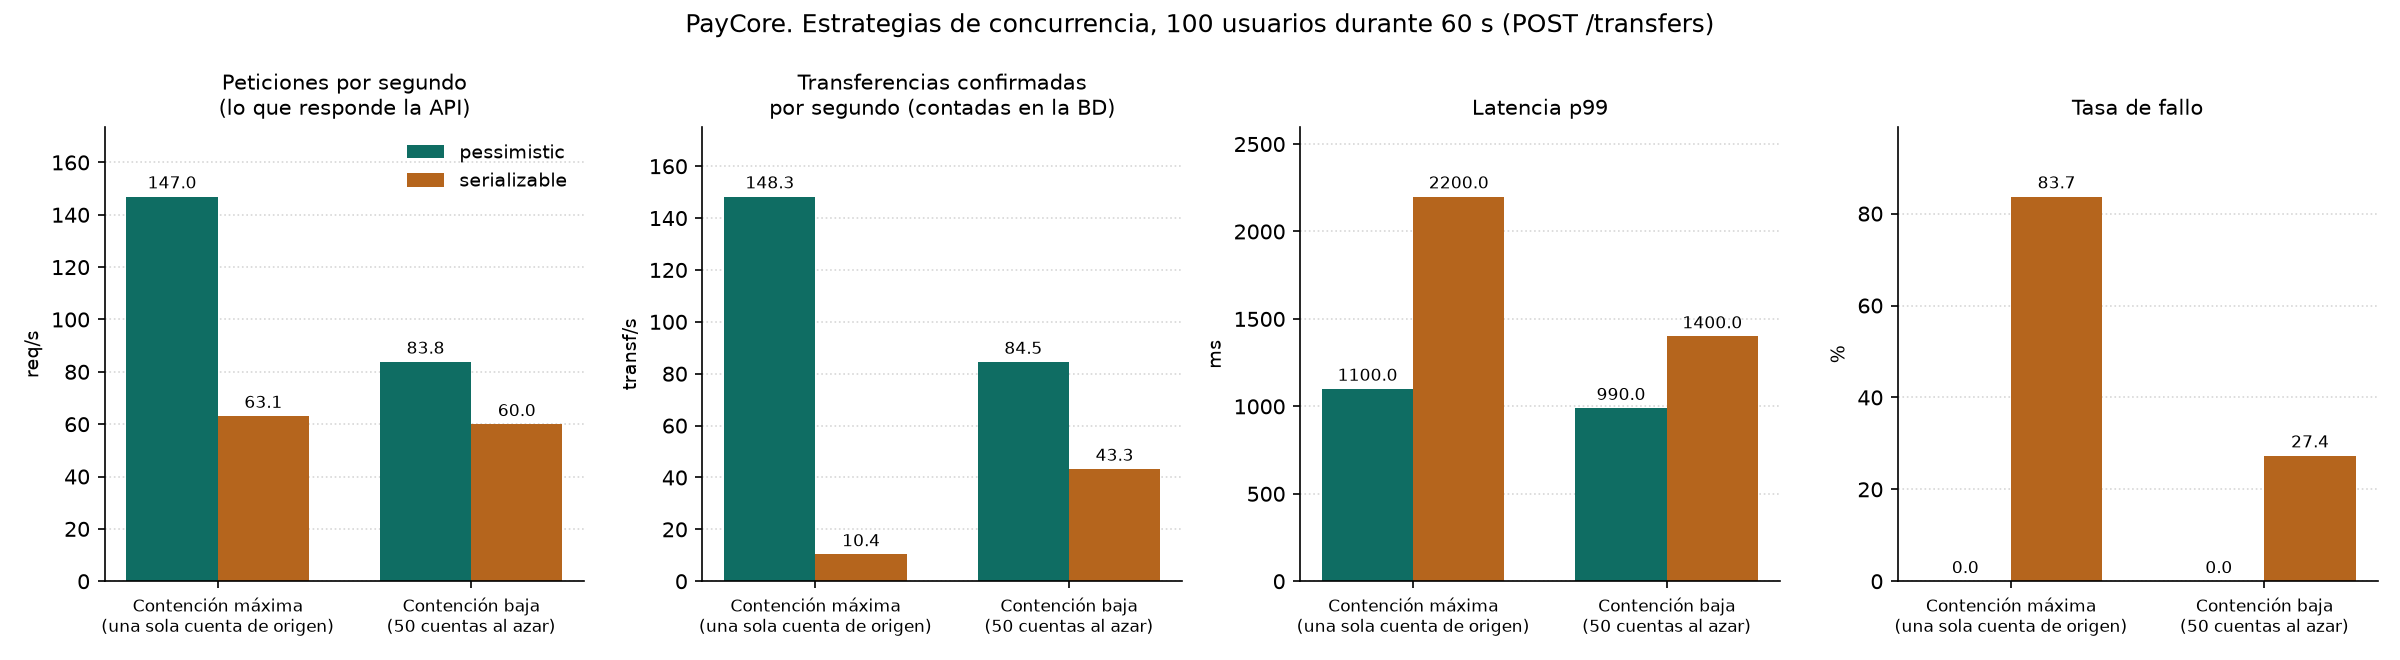
\includegraphics[width=\textwidth]{../diagrams/rendimiento-estrategias.png}
\caption{Estrategias de concurrencia bajo cien usuarios durante sesenta
segundos. El segundo panel es el que cuenta el trabajo realmente hecho.}
\label{fig:estrategias}
\end{figure}

\begin{figure}[htbp]
\centering
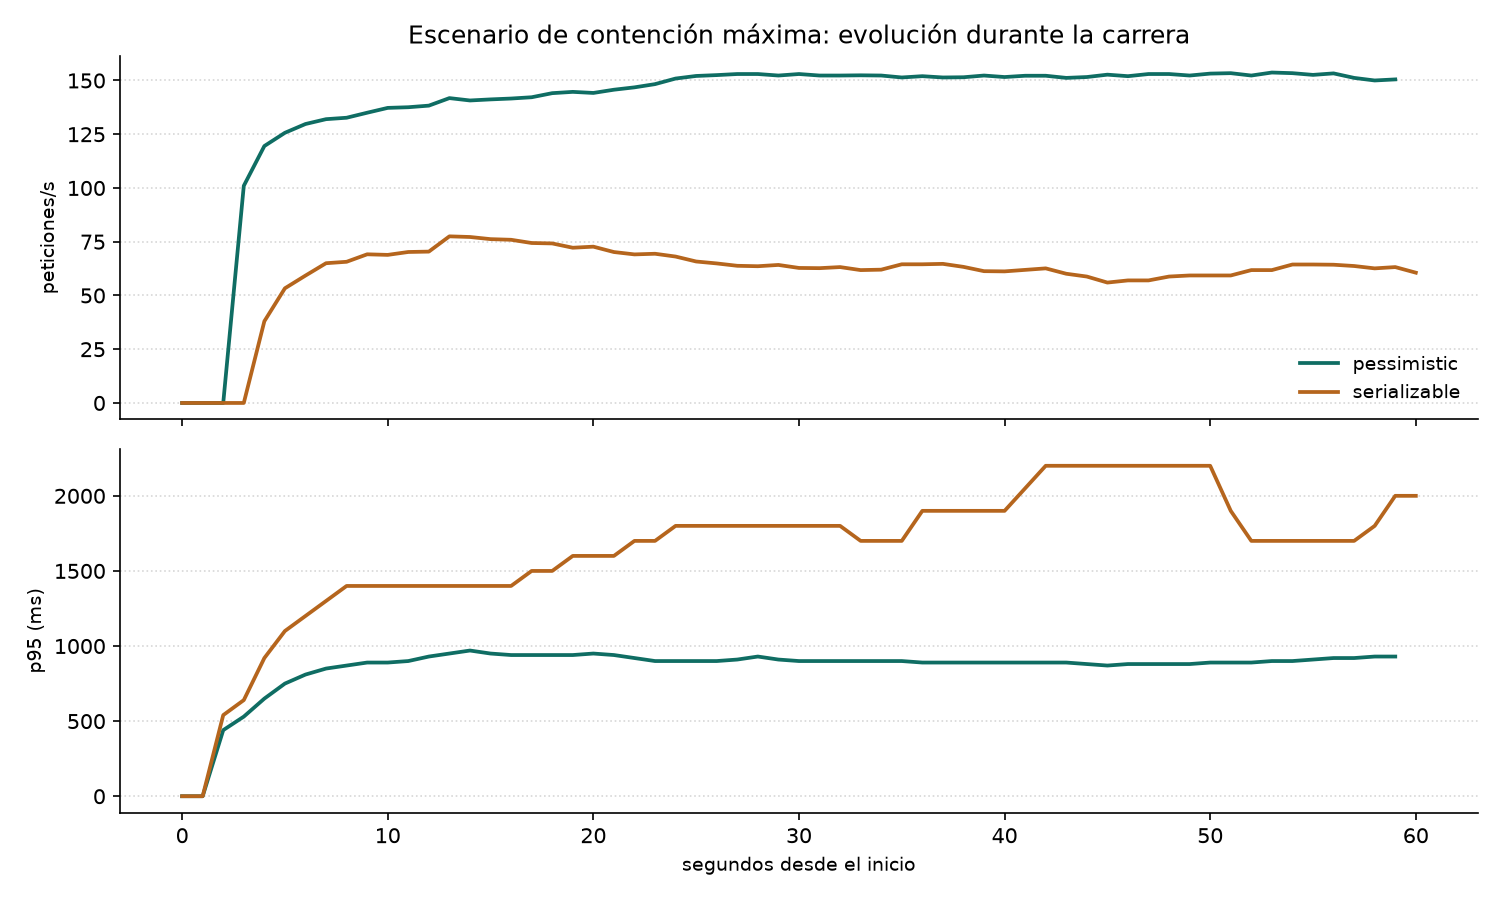
\includegraphics[width=\textwidth]{../diagrams/rendimiento-serie-temporal.png}
\caption{Evolución durante la carrera en el escenario de contención máxima.
Las dos estrategias alcanzan su régimen estacionario en los primeros segundos
y se mantienen: no hay degradación progresiva ni fuga de conexiones.}
\label{fig:serie}
\end{figure}

\subsection{Una optimización medida antes y después}
\label{subsec:optimizacion}

\paragraph{El síntoma.} La carrera de solo lectura daba menos peticiones por
segundo que el escenario mixto, que hace más trabajo, con fallos y un
percentil 95 de 30\,000\,ms. El registro señalaba la causa sin ambigüedad:
\codigo{QueuePool limit of size 10 overflow 10 reached, connection timed out,
timeout 30.00}.

\paragraph{Primera capa del diagnóstico.} Los endpoints son síncronos, así
que se ejecutan en el grupo de hilos de AnyIO, que por defecto admite cuarenta
simultáneos, mientras que el pool de cada worker entregaba como mucho veinte
conexiones. El límite de concurrencia de la aplicación y la capacidad del pool
eran dos números fijados por separado que deberían haber sido el mismo. Se
igualaron en el arranque y se bajó el tiempo de espera del pool a cinco
segundos, para fallar rápido con un 503 en lugar de dejar al cliente colgado
medio minuto. \textbf{No bastó.}

\paragraph{Segunda capa, la de verdad.} La sesión de base de datos se obtenía
como \emph{dependencia del framework}. Una dependencia se abre antes de entrar
en la función y se cierra después de salir, por lo que la conexión queda
retenida en tramos en los que la petición ya no ocupa ningún hilo. El número
de conexiones en uso podía por tanto superar al de hilos activos. La
corrección fue acotar la sesión al cuerpo del endpoint con un gestor de
contexto, de modo que cada conexión vive exactamente lo que vive su hilo.

\begin{table}[htbp]
\centering
\caption{Efecto de acotar la sesión al cuerpo del endpoint. Las dos carreras
se hicieron seguidas, con 59 s reales cada una y la misma carga.}
\label{tab:optimizacion}
\small
\begin{tabular}{@{}lrr@{}}
\toprule
\textbf{Métrica} & \textbf{Antes} & \textbf{Después} \\
\midrule
\codigo{GET /accounts/me/balance}, peticiones/s & 8,8 & 76,3 \\
Agregado de los dos endpoints de lectura & 20,8 & 154,6 \\
p50 & 270 ms & 580 ms \\
p95 & 30\,000 ms & 780 ms \\
p99 & 31\,000 ms & 840 ms \\
Máximo observado & 30\,664 ms & 1\,100 ms \\
Tasa de fallo & 3,25\,\% & 0,00\,\% \\
\bottomrule
\end{tabular}
\end{table}

\begin{figure}[htbp]
\centering
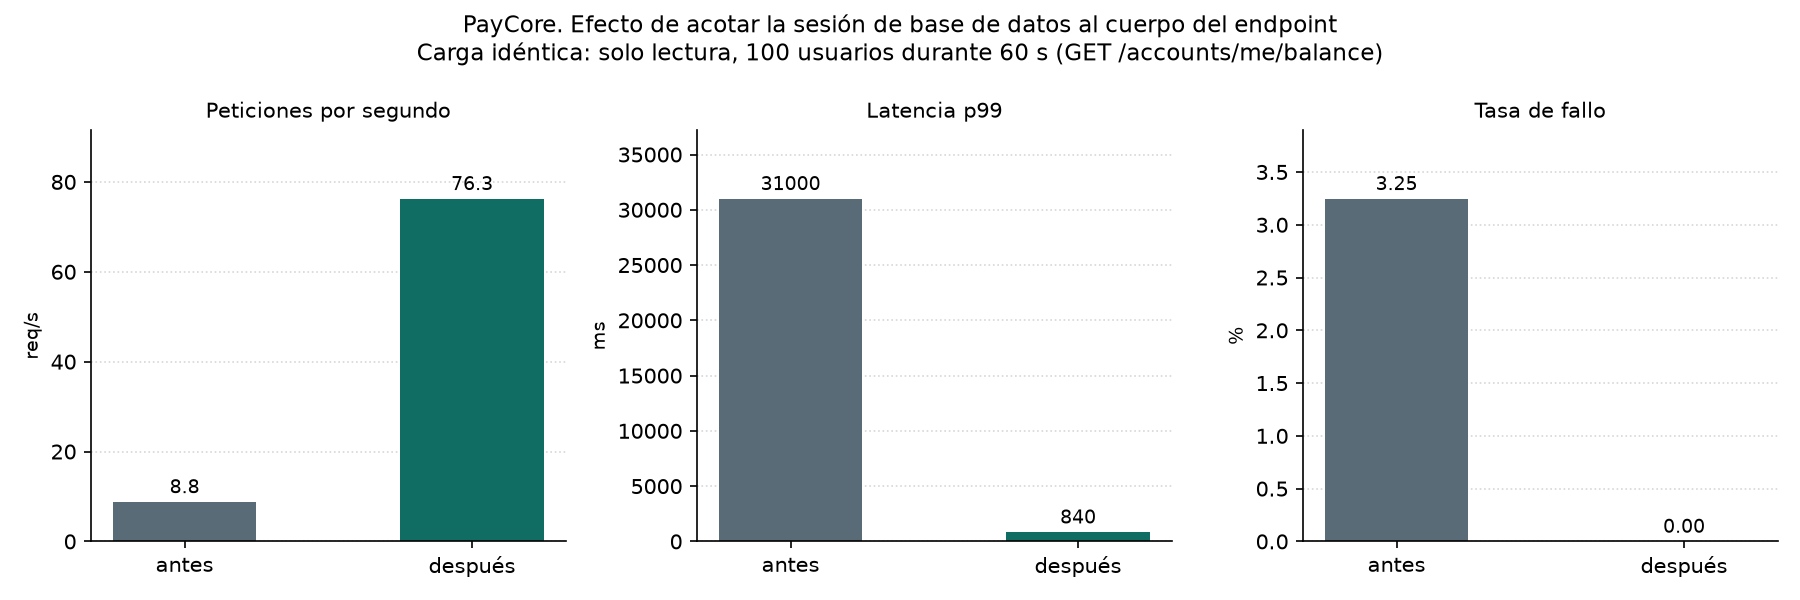
\includegraphics[width=\textwidth]{../diagrams/rendimiento-optimizacion.png}
\caption{Antes y después de la corrección, con carga idéntica.}
\label{fig:optimizacion}
\end{figure}

El rendimiento agregado se multiplica por 7,4 y la cola desaparece. Merece la
pena mirar el p50, que \textbf{sube} de 270 a 580\,ms: no es un empeoramiento,
es lo que ocurre cuando el sistema deja de descartar trabajo. Antes la mediana
solo medía a las pocas peticiones afortunadas que conseguían conexión enseguida
mientras el resto se atascaba o fallaba. Es justo el motivo por el que este
informe reporta percentiles y nunca la media sola.

\subsection{Una medición que hubo que descartar}

El primer intento de esta comparación no era válido y no se publica. La
carrera del \enquote{antes} había durado \textbf{34 segundos y no 60}, porque
el generador de carga de entonces abortaba la ejecución cuando fallaba un
inicio de sesión. Las peticiones por segundo que reportó la consola y las que
quedaron en el CSV ni siquiera coincidían entre sí, precisamente porque se
calculaban sobre ventanas de tiempo distintas de una carrera truncada.

Se detectó al comprobar las marcas de tiempo del historial antes de escribir
esta sección. Se corrigió el generador para que un inicio de sesión fallido
sea un dato y no un motivo de aborto, y se repitió la medición completa. Queda
anotado porque una cifra que no se puede defender es peor que no tener cifra.

\section{Análisis de resultados}
\label{sec:resultados}

\subsection{Las dos estrategias son igual de correctas}

En las cuatro carreras de escritura, bajo cien usuarios durante sesenta
segundos y con cuatro procesos compitiendo, la verificación contra PostgreSQL
dio siempre lo mismo: suma global del libro mayor igual a cero, cero cuentas
descuadradas y cero saldos negativos. Ese es el resultado que el proyecto
quería demostrar, y es independiente de la estrategia empleada.

Dicho de otro modo: las garantías no dependen de haber elegido bien entre
bloqueo pesimista y \codigo{SERIALIZABLE}. Dependen de que las invariantes
vivan en el motor y de que la transferencia sea una sola transacción.

\subsection{Se diferencian en cuánto trabajo terminan}

Bajo contención máxima, la estrategia pesimista confirma 148,3 transferencias
por segundo y \codigo{SERIALIZABLE} solo 10,4. Catorce veces menos, aunque su
tasa de peticiones por segundo (63,1 frente a 147,0) sugiera una diferencia
mucho menor. La explicación está en la columna de fallos: el 83,72\,\% de las
peticiones termina en un 503 porque se agotan los tres reintentos ante
\sqlstate{40001}.

\subsection{La conclusión depende de dónde se mire}

Este es el hallazgo metodológico de la fase. Si el análisis se hubiera quedado
en las peticiones por segundo que reporta el generador de carga, la conclusión
habría sido \enquote{\codigo{SERIALIZABLE} rinde un 57\,\% menos}. Contando
las filas realmente escritas en PostgreSQL, la conclusión es que hace un
93\,\% menos de trabajo útil.

Son dos afirmaciones muy distintas sobre el mismo sistema, y solo una es
cierta. Medir la respuesta de la API y verificar que las transacciones se
registraron no son la misma cosa, y confundirlas es fácil.

\subsection{Comparación con la literatura}

Ports y Grittner reportan para su implementación un coste inferior al 7\,\%
respecto al aislamiento por instantáneas~\cite{ports2012}. Las mediciones de
PayCore bajo contención máxima arrojan una diferencia mucho mayor. No hay
contradicción, y la razón importa:

\begin{itemize}[leftmargin=1.2em]
  \item Sus cargas de evaluación reparten el trabajo entre muchas filas. El
    escenario \codigo{caliente} de PayCore concentra \emph{todas} las
    escrituras en una sola fila, que es el peor caso concebible para una
    estrategia optimista.
  \item Su cifra mide el coste de la \emph{técnica} cuando los conflictos son
    raros. La de PayCore mide el efecto de los \emph{conflictos} cuando son
    constantes.
  \item En el escenario de contención baja, con cien usuarios sobre cincuenta
    cuentas, la diferencia se reduce pero no desaparece: sigue habiendo un
    27,35\,\% de fallos. Haría falta una dispersión mucho mayor para que
    \codigo{SERIALIZABLE} compitiera, y ese no es el perfil de carga de una
    billetera.
\end{itemize}

\subsection{Verificación de la hipótesis previa}

El registro de decisión sobre concurrencia declaró, \emph{antes} de medir, que
bajo contención máxima se esperaba que la estrategia optimista degenerase en
abortos y reintentos. La medición lo confirma. La hipótesis estaba escrita con
fecha anterior a los datos, lo que permite distinguir una predicción acertada
de una racionalización posterior.

\subsection{Qué aportó cada tipo de prueba}

\begin{table}[htbp]
\centering
\caption{Defectos reales encontrados, y por qué tipo de prueba.}
\label{tab:hallazgos}
\small
\begin{tabularx}{\textwidth}{@{}lXX@{}}
\toprule
\textbf{Tipo} & \textbf{Qué encontró} & \textbf{Por qué nada más lo veía} \\
\midrule
Unitarias y de integración & Nada que las de concurrencia no vieran después &
  Un solo hilo nunca reproduce una carrera \\
Concurrencia & La actualización perdida del mapa de identidad: 88
  transferencias aprobadas de 100 &
  Las 76 pruebas existentes pasaban todas con el defecto presente \\
Carga & El agotamiento del pool de conexiones por retener la sesión fuera del
  hilo & Solo aparece con suficientes peticiones simultáneas y rápidas \\
Revisión de la propia medición & Una carrera truncada a 34 s que invalidaba
  una comparación & Los totales parecían razonables; solo las marcas de
  tiempo lo delataban \\
\bottomrule
\end{tabularx}
\end{table}

La lectura de este cuadro es la conclusión práctica del proyecto: cada tipo de
prueba encuentra una clase de defecto que las demás no pueden ver, y eso
incluye revisar críticamente las propias mediciones.

\section{Limitaciones}
\label{sec:limitaciones}

Se enumeran por escrito, en el informe y en el repositorio, porque conocerlas
es parte del trabajo y porque la alternativa, dejarlas implícitas, convertiría
el proyecto en algo que no es.

\subsection{Del sistema}

\begin{description}[leftmargin=0.6cm,style=nextline]
  \item[Un solo nodo de base de datos.] Sin alta disponibilidad ni
    replicación. Es un punto único de fallo y el techo de escritura es el de
    una instancia.
  \item[La limitación de peticiones cuenta en memoria del proceso.] Con cuatro
    workers, la ráfaga efectiva del inicio de sesión es veinte y no cinco.
    Resolverlo exige un contador compartido.
  \item[Tokens sin revocación inmediata.] Un token robado es válido hasta que
    caduca. Se mitiga con una vida de quince minutos; la solución completa es
    una lista de revocación o sesiones en base de datos.
  \item[El token del navegador vive en \codigo{sessionStorage}.] Se borra al
    cerrar la pestaña, pero cualquier ataque de tipo \emph{cross-site
    scripting} podría leerlo. La respuesta correcta en producción es una
    cookie \codigo{httpOnly} con protección contra falsificación de petición
    entre sitios.
  \item[Una cuenta por usuario.] El modelo admite varias, pero el MVP impone
    una por unicidad.
  \item[Docker Compose no es un despliegue de producción.] No hay
    orquestación, ni secretos gestionados, ni cifrado en reposo.
  \item[Sin observabilidad continua.] Hay registro estructurado y correlación,
    pero no métricas exportadas ni trazas distribuidas.
\end{description}

\subsection{De las mediciones}

\begin{description}[leftmargin=0.6cm,style=nextline]
  \item[Cliente y servidor en la misma máquina.] El generador de carga, los
    cuatro workers y PostgreSQL compiten por los mismos dieciséis hilos de
    CPU. Los números absolutos serían distintos con la carga generada desde
    fuera; las comparaciones entre estrategias, que es para lo que se
    hicieron, sí son válidas porque todas sufren la misma interferencia.
  \item[Omisión coordinada.] Locust es un generador de bucle cerrado: cuando
    el servidor se ralentiza deja de emitir peticiones, de modo que las
    latencias altas quedan subrepresentadas. Las cifras de cola son por tanto
    optimistas.
  \item[Un minuto por carrera.] Suficiente para el régimen estacionario,
    insuficiente para ver efectos lentos como el crecimiento de las tablas o
    el comportamiento del recolector de versiones.
  \item[Sin medición de recursos.] No se registró uso de CPU ni de memoria por
    proceso. Queda como pendiente, no como dato estimado.
  \item[Una sola repetición por combinación.] No hay intervalos de confianza.
    Las diferencias que se discuten son lo bastante grandes como para no
    depender del ruido, pero las pequeñas no deberían interpretarse.
  \item[La carga ambiente varía entre carreras.] Una misma configuración
    medida en dos momentos distintos dio 280,6 y 154,6 peticiones por segundo
    en el escenario de lectura. Por eso las comparaciones del
    apartado~\ref{subsec:optimizacion} se hicieron con las dos carreras
    seguidas.
  \item[No es una prueba de capacidad.] No se buscó el punto de saturación ni
    la carga máxima sostenible.
\end{description}

\subsection{Del alcance}

PayCore no implementa conciliación con entidades externas, ni reversiones
contables, ni límites regulatorios, ni prevención de blanqueo, ni
notificaciones, ni recuperación de contraseña, ni verificación de identidad.
Nada de eso está a medias: directamente no existe, y decirlo es más útil que
insinuar lo contrario.

\section{Trabajo futuro}
\label{sec:futuro}

Se ordena por el criterio que gobierna todo el proyecto: cada incorporación
tiene que resolver un problema observado, no sonar avanzada.

\subsection{Lo que arreglaría limitaciones ya conocidas}

\begin{description}[leftmargin=0.6cm,style=nextline]
  \item[Contador de limitación compartido.] En cuanto el despliegue pase de un
    proceso, el límite actual deja de significar lo que dice. Es la condición
    escrita de reingreso de Redis, donde sí resolvería un problema real sin
    romper ninguna garantía transaccional.
  \item[Revocación de tokens.] Una lista de revocación consultada por
    identificador de token, o el paso a sesiones en base de datos si la
    revocación inmediata se vuelve un requisito.
  \item[Cookie \codigo{httpOnly} para el navegador.] Exige que la API y el
    frontend compartan origen, y protección contra falsificación de petición
    entre sitios.
  \item[Réplica de lectura.] Las consultas de saldo e historial no necesitan
    la instancia primaria. Antes de hacerlo habría que medir si la lectura es
    realmente el cuello de botella; con los datos actuales no lo es.
  \item[Medición de recursos.] Instrumentar CPU y memoria por proceso durante
    las carreras, para completar lo que la sección~\ref{sec:rendimiento} deja
    pendiente.
\end{description}

\subsection{Lo que ampliaría el alcance}

\begin{description}[leftmargin=0.6cm,style=nextline]
  \item[Reversiones contables.] Una transferencia errónea no se borra: se
    compensa con un asiento de reversión. El libro mayor de solo inserción ya
    está preparado para ello; falta el caso de uso y su autorización.
  \item[Varias cuentas por usuario.] El modelo lo admite y la autorización ya
    está escrita para el caso general; solo habría que levantar la
    restricción de unicidad y ajustar la interfaz.
  \item[Fracciones de céntimo.] Si alguna vez hicieran falta intereses o
    comisiones prorrateadas, la vía es \codigo{NUMERIC} con una política de
    redondeo explícita, nunca punto flotante.
  \item[Arquitectura orientada a eventos para lo posterior.] Notificaciones,
    puntuación de riesgo y analítica son consumidores naturales del libro
    mayor. La transferencia seguiría siendo síncrona y atómica.
\end{description}

\subsection{Inteligencia artificial, con condiciones}

El límite de diseño es permanente: \textbf{ningún modelo aprueba, rechaza ni
modifica una transferencia o un saldo}. Dentro de ese límite:

\begin{enumerate}[leftmargin=1.4em]
  \item \textbf{Reglas deterministas de riesgo} (velocidad de envío, importe
    atípico frente al historial propio, receptor nuevo) que adjunten una marca
    de revisión. Son baratas, explicables y auditables, y es lo que un sistema
    real pone primero.
  \item \textbf{Detección de anomalías no supervisada} como experimento, con
    la etiqueta explícita de que los datos son sintéticos y el resultado no es
    generalizable.
  \item Un clasificador supervisado de fraude \textbf{no} entra: necesitaría
    transacciones reales etiquetadas, que no existen y no se pueden fabricar
    sin falsear el resultado~\cite{sculley2015}.
\end{enumerate}

\section{Conclusiones}
\label{sec:conclusiones}

\subsection{Sobre los objetivos}

Los ocho objetivos específicos de la sección~2 se cumplieron, y siete de los
ocho tienen verificación automatizada asociada. Las seis pruebas funcionales
exigidas pasan, y todas comprueban el resultado en la base de datos en lugar
de en las respuestas HTTP.

\subsection{Sobre las garantías}

La conclusión técnica central es que \textbf{las garantías de integridad no
dependieron de la estrategia de concurrencia elegida}. En las cuatro carreras
de escritura, con cien usuarios durante sesenta segundos y cuatro procesos
compitiendo, el libro mayor sumó exactamente cero, ninguna cuenta quedó
descuadrada y ningún saldo resultó negativo, tanto con bloqueo pesimista como
con \codigo{SERIALIZABLE}.

Lo que sí dependió de la estrategia fue cuánto trabajo se completó: 148,3
frente a 10,4 transferencias confirmadas por segundo bajo contención máxima.
Corrección y rendimiento resultaron ser dimensiones separables, y conviene no
confundirlas al justificar una decisión.

\subsection{Sobre dónde deben vivir las invariantes}

Nueve de las diez invariantes del sistema se aplican en PostgreSQL y no en
Python. Las diecisiete pruebas de esquema las atacan con SQL directo, sin
pasar por la aplicación: si alguna viviera solo en el código, esas pruebas se
pondrían rojas.

Esa decisión tuvo un rendimiento concreto. La restricción de no negatividad
nunca llegó a dispararse durante la actualización perdida, porque el saldo
calculado a partir del valor obsoleto no cruzaba el cero. Una restricción de
motor acota el daño, pero no sustituye a la prueba. Ambas cosas eran
necesarias.

\subsection{Sobre el método}

Los dos defectos más valiosos del proyecto no los encontró la revisión de
código, sino las pruebas que ejercitan el sistema en las condiciones en las
que falla:

\begin{itemize}[leftmargin=1.2em]
  \item La \textbf{prueba de concurrencia} destapó una actualización perdida
    con la que las 76 pruebas existentes pasaban todas. Tomar el bloqueo
    correcto en SQL no basta si la capa de mapeo devuelve datos cacheados.
  \item La \textbf{prueba de carga} destapó un agotamiento del pool de
    conexiones causado por retener la sesión fuera del hilo que la usaba.
    Corregirlo multiplicó por 7,4 el rendimiento de lectura.
\end{itemize}

A eso se añade una tercera lección, menos cómoda: una de las mediciones de
este informe hubo que descartarla por no ser válida. Revisar críticamente los
propios datos antes de publicarlos resultó ser tan necesario como medirlos.

\subsection{Sobre lo que no se hizo}

PayCore no incorpora Redis, ni Kafka, ni Kubernetes, ni microservicios, ni
modelos de aprendizaje automático. Para cada uno está escrita la condición
concreta bajo la cual entraría. Esa lista de exclusiones, con su justificación
y su condición de reingreso, es tan parte del diseño como lo que sí se
construyó: una decisión técnica no se defiende solo explicando lo que se
eligió, sino también lo que se descartó y por qué.

\subsection{Valoración final}

El sistema cumple su propósito: demostrar, con pruebas reproducibles y
mediciones propias, que las garantías que un motor de pagos debe ofrecer se
pueden construir y verificar. No es una plataforma bancaria de producción y el
informe dedica una sección entera a explicar por qué no lo es. Entre un
prototipo que exagera lo que hace y uno que delimita con precisión lo que
garantiza, el segundo es el que se puede defender.


\clearpage
\printbibliography[title={Referencias bibliográficas},heading=bibnumbered]

\end{document}
